\documentclass[pdflatex,sn-mathphys-num]{sn-jnl}

% ============================================================
% MEDICORE RESEARCH MANUSCRIPT & COMPREHENSIVE TECHNICAL REPORT
% Blockchain-Based Pharmaceutical Supply Chain Management
% ============================================================

\usepackage{graphicx}
\usepackage{multirow}
\usepackage{amsmath,amssymb,amsfonts}
\usepackage{amsthm}
\usepackage{booktabs}
\usepackage{array}
\usepackage{tabularx}
\usepackage{url}
\usepackage{xcolor}
\usepackage{enumitem}
\usepackage{tikz}
\usetikzlibrary{shapes.geometric, arrows.meta, positioning, calc}
\usepackage{pgfplots}
\usepackage{float}
\usepackage{listings}
\usepackage{caption}
\usepackage{subcaption}

\pgfplotsset{compat=1.18}

% Configure graphics paths for seamless Overleaf / local compilation
\graphicspath{{paperassets/}{./}{images/}{docs/screenshots/}}

% Define Theorem Environments
\theoremstyle{thmstyleone}
\newtheorem{theorem}{Theorem}
\newtheorem{proposition}[theorem]{Proposition}
\newtheorem{lemma}[theorem]{Lemma}

\theoremstyle{thmstyletwo}
\newtheorem{example}{Example}
\newtheorem{remark}{Remark}

\theoremstyle{thmstylethree}
\newtheorem{definition}{Definition}

\raggedbottom

% ============================================================
% DOCUMENT INFORMATION
% ============================================================

\begin{document}

\title[MEDICORE: Intelligent Blockchain Pharmaceutical Supply Chain]{MEDICORE: An Intelligent Blockchain-Based Framework for Pharmaceutical Supply Chain Traceability, Verification, and Anomaly Monitoring}

% ============================================================
% AUTHORS
% ============================================================

\author*[1]{\fnm{Aditya Kumar} \sur{Roy}}\email{2301020723@cgu-odisha.ac.in}
\author[1]{\fnm{Krishna} \sur{Das}}\email{2302020839@cgu-odisha.ac.in}

\affil*[1]{
\orgdiv{Department of Computer Science and Engineering},
\orgname{C. V. Raman Global University},
\orgaddress{
\street{Bidyanagar, Mahura, Janla},
\city{Bhubaneswar},
\state{Odisha},
\postcode{752054},
\country{India}
}
}

% ============================================================
% ABSTRACT
% ============================================================

\abstract{
Global pharmaceutical supply chains require mathematically verifiable traceability, strictly controlled ownership transitions, accessible product verification, continuous cold-chain monitoring, and rapid, synchronized responses to multi-jurisdictional recalls. Conventional pharmaceutical systems distribute custody records across fragmented, siloed Enterprise Resource Planning (ERP) databases, introducing substantial vulnerabilities including administrative data alteration, counterfeit infiltration, illicit diversion, unrecorded thermal excursions, and catastrophic custodial blind spots. This paper presents \textbf{MEDICORE}, a comprehensive, enterprise-grade blockchain framework engineered to unify entity identity governance, production batch minting, laboratory quality approvals, physical shipment routing, cryptographic zero-trust handoffs, automated recall propagation, IoT cold-chain monitoring, and real-time anomaly detection into an integrated operational architecture.

MEDICORE employs Solidity smart contracts deployed on the Ethereum Virtual Machine (EVM) for authorization-critical and traceability-sensitive state transitions, while high-frequency operational telemetry (real-time GPS streaming and ambient sensor logs) is ingested off-chain via an asynchronous Node.js/Express sentinel service backed by SQLite. The protocol establishes permanent digital entity identifiers logically decoupled from mutable cryptographic wallet addresses, verifiable Digital Product Passports (DPPs), strict EVM-level mathematical quantity conservation ($\sum Q_{\text{minted}} = Q_{\text{remaining}} + Q_{\text{transferred}} + Q_{\text{quarantined}}$), Keccak-256 secret-preimage delivery handoffs, role-based access control (RBAC) across seven operational tiers, and explainable multi-signal anomaly risk vectors. Crucially, zero-wallet client interfaces permit end consumers to independently audit complete provenance and packaging integrity via read-only JSON-RPC queries without requiring cryptocurrency, browser extensions, or Web3 onboarding.

The framework is empirically validated through the complete implemented prototype dataset (encompassing seven supply-chain entities, five pharmaceutical batches, eight custody transfer transactions, and active recall/cold-chain excursion scenarios), automated smart contract test suites, and comprehensive local EVM execution benchmarks. The prototype executes batch minting at 186,412 gas, shipment creation at 124,310 gas, and cryptographic receipt at 94,820 gas, while delivering sub-10 ms public verification latency (9.55 ms) and 100\% enforcement of role-based authorization constraints. We further present extensive implementation visual evidence encompassing all eleven operational command centers and dashboards, evaluate security against adversarial threat vectors, and provide a critical analysis of current cyber-physical limitations to guide next-generation production deployments.
}

\keywords{
Blockchain,
Pharmaceutical Supply Chain,
Drug Traceability,
Smart Contracts,
Digital Product Passport,
QR Verification,
Cold Chain Telemetry,
GPS Tracking,
Anomaly Detection,
Zero-Trust Handoff,
Ethereum Virtual Machine,
Supply Chain Intelligence
}

\maketitle

% ============================================================
% 1. INTRODUCTION
% ============================================================

\section{Introduction}\label{sec:introduction}

The pharmaceutical supply chain is one of the most critical socio-technical infrastructures supporting modern public health. However, the international distribution of genuine, life-saving therapeutics is severely undermined by fraudulent counterfeiting, cargo theft, unauthorized geographic diversion, and unmonitored cold-chain temperature excursions. According to comprehensive field assessments conducted by the World Health Organization (WHO), substandard and falsified (SF) medical products represent an estimated 10.5\% of all circulating pharmaceuticals across low- and middle-income nations, resulting in upwards of one million preventable fatalities annually and causing severe antimicrobial resistance across vulnerable populations \cite{who2024substandard,who2017substandard}. Economically, the counterfeit drug trade generates over \$430 billion in annual illicit revenue, representing the most lucrative sector of global intellectual property crime \cite{mackey2020blockchain}.

In parallel with counterfeit infiltration, modern biopharmaceuticals, including mRNA vaccines, insulin analogs, and monoclonal antibodies, demand uncompromised cold-chain maintenance within strict thermal envelopes (typically $2^\circ\text{C}$ to $8^\circ\text{C}$ or ultra-cold frozen conditions). When thermal integrity is compromised during inter-facility transit or intermediate cross-docking, biological proteins undergo denaturation, leading to potency degradation and hazardous immunological toxicity \cite{tsang2018iot,hosseini2021blockchain}. Industry analyses indicate that cold-chain thermal failures result in more than \$35 billion in annual biopharmaceutical losses globally.

\subsection{Architectural Deficiencies of Centralized Systems}

Contemporary pharmaceutical logistics relies almost universally on centralized Enterprise Resource Planning (ERP) databases, proprietary electronic data interchange (EDI) message buses, and centralized GS1-compliant serialization repositories. Although technologically mature within individual corporate perimeters, centralized architectures exhibit fundamental architectural limitations when coordinating multi-stakeholder supply chains:

\begin{enumerate}[label=(\roman*)]
    \item \textbf{Single Points of Trust and Administrative Vulnerability:} Centralized relational databases rely on privileged system administrators. Malicious insiders, compromised credentials, or state-sponsored attackers can alter historical batch records, modify manufacturing timestamps, or erase inventory balances without cryptographic auditability \cite{clauson2018leveraging}.
    \item \textbf{Opaque Cross-Organizational Custodial Transitions:} In complex distribution pipelines spanning primary manufacturers, freight forwarders, third-party logistics (3PL) carriers, regional wholesalers, and retail pharmacies, physical product custody transfers are recorded via isolated paper shipping manifests or incompatible private ERP instances. These systemic blind spots are exploited by black-market intermediaries to inject counterfeit medications into legitimate distribution channels.
    \item \textbf{Lack of Zero-Wallet Consumer Verification:} Existing serialization initiatives (e.g., the United States Drug Supply Chain Security Act [DSCSA] and European Union Falsified Medicines Directive [EU FMD]) mandate 2D DataMatrix barcodes. However, verification is restricted to authorized trading partners. End patients and healthcare practitioners possess no trustless mechanism to independently verify drug provenance without blindly trusting centralized web portals.
    \item \textbf{Decoupled and Reactive Cold-Chain Auditing:} Traditional passive USB temperature dataloggers are evaluated only upon final cargo arrival. If an excursion occurred during early-stage transport, compromised batches frequently sit in regional warehouses before manual inspection, lacking autonomous on-chain quarantine mechanisms.
\end{enumerate}

\subsection{Research Objectives and Contributions}

To address these systemic vulnerabilities, this work presents \textbf{MEDICORE}, a holistic, decentralized pharmaceutical supply-chain framework that combines EVM-based smart contracts with an intelligent off-chain telemetry sentinel, cryptographic delivery verification, and zero-wallet consumer access. MEDICORE is architected around five core technical objectives:
\begin{enumerate}
    \item Establishing permanent, immutable digital identities for all network stakeholders, decoupled from mutable cryptographic keypairs.
    \item Enforcing strict on-chain mathematical quantity conservation to eliminate digital token duplication and unauthorized inventory creation.
    \item Implementing a zero-trust cryptographic handoff protocol based on Keccak-256 hash commitments to decouple physical freight transport from digital ownership.
    \item Developing an asynchronous, explainable anomaly-monitoring engine capable of detecting route deviations, thermal excursions, and brute-force QR verification attacks.
    \item Delivering a public, zero-wallet Digital Product Passport (DPP) interface operating via read-only JSON-RPC queries.
\end{enumerate}

The principal contributions of this work are summarized as follows:
\begin{itemize}
    \item \textbf{Decentralized Multi-Tier Governance:} A Solidity smart contract architecture implementing seven distinct supply-chain operational roles and an emergency administrative kill-switch.
    \item \textbf{Mathematical Inventory Invariance:} Formal specification and proof of an EVM-enforced quantity conservation invariant ensuring that physical stock movements balance ledger allocations at all discrete state transitions.
    \item \textbf{Cryptographic Anti-Diversion Handoff:} A single-use delivery secret mechanism ensuring that transporters cannot forge deliveries and receiving entities cannot claim stock without physical possession of the carrier's secret.
    \item \textbf{Dual-Consensus Recall Protocol:} A 2-of-$N$ multi-signature consensus workflow requiring joint authorization between pharmaceutical manufacturers and regulatory agencies to execute global batch recalls.
    \item \textbf{Empirical System Validation:} A comprehensive experimental benchmark utilizing the actual prototype deployment on a local EVM network, reporting gas metrics, verification latencies, and complete implementation visual evidence across eleven system interfaces.
\end{itemize}

% ============================================================
% 2. RELATED WORK
% ============================================================

\section{Related Work}\label{sec:related-work}

The convergence of distributed ledger technology (DLT), IoT sensor networks, and supply-chain management has generated extensive academic and industrial investigation over the past decade.

\subsection{Blockchain in Supply Chain Provenance}

The seminal foundations of decentralized ledgers established by Nakamoto \cite{nakamoto2008bitcoin} and smart contract primitives formalized by Szabo \cite{szabo1997formalizing} introduced decentralized mechanisms for multi-party coordination without trusted intermediaries. Early surveys by Crosby et al. \cite{crosby2016blockchain} and Casino et al. \cite{casino2019systematic} categorized blockchain applications across financial and non-financial domains, highlighting supply-chain provenance as an ideal application of append-only, tamper-evident data structures. Subsequent studies by Kamilaris et al. \cite{kamilaris2019rise}, Saberi et al. \cite{saberi2019blockchain}, Queiroz et al. \cite{queiroz2020blockchain}, and Wang et al. \cite{wang2019understanding} analyzed the operational drivers, organizational adoption barriers, and sustainability benefits of distributed supply chains.

In the healthcare domain, Liu et al. \cite{liu2021blockchain} proposed a blockchain-based tracking and tracing platform utilizing smart contracts to monitor pharmaceutical batch lifecycles. Similarly, Musamih et al. \cite{musamih2021blockchain} implemented an Ethereum-based drug traceability system utilizing smart contract events to reconstruct provenance trails. However, these foundational frameworks primarily focused on token transfers, failing to address the mathematical conservation of bulk pharmaceutical inventory when batches are dynamically split across multiple regional wholesalers.

\subsection{Permissioned vs. Permissionless Architectures}

A major architectural debate centers on the selection between permissioned ledgers (e.g., Hyperledger Fabric) and permissionless/EVM-compatible frameworks. Naga Sudha and Nayahi \cite{nagasudha2024trackchain} introduced \textit{TrackChain}, a Hyperledger-based pharmaceutical supply-chain architecture prioritizing resource efficiency and transaction throughput. While permissioned blockchains offer high write throughput and eliminate cryptocurrency gas fees, they suffer from significant practical limitations: they depend on centralized Certificate Authorities (CAs) to grant public key certificates, restricting public access. Patients and independent pharmacies cannot verify medications without explicit network onboarding.

Conversely, public and EVM-compatible architectures (such as Ethereum Layer-1 and Layer-2 rollups) provide open access. Akram et al. \cite{akram2024blockchain} provided a comprehensive review of blockchain applications in pharmaceutical supply chains, emphasizing that hybrid architectures—combining private write permissions for licensed commercial actors with open, read-only verification for the public—represent the most viable model for global healthcare compliance. Henrichs et al. \cite{henrichs2025quantum} introduced the ``Quantum of Trust'' taxonomy, demonstrating that physical product authentication requires decoupling digital ledger proofs from physical packaging identifiers.

\subsection{IoT-Enabled Cold-Chain Monitoring}

The integration of IoT sensor telemetry with blockchain ledgers introduces physical observation to digital provenance. Yadav et al. \cite{yadav2022blockchain} explored adoption barriers in vaccine supply chains, emphasizing the vulnerability of temperature-sensitive biologics in developing nations. Antal et al. \cite{antal2018blockchain} demonstrated an automated cold-chain management framework executing smart contract actions upon threshold violations. Mutambik \cite{mutambik2026blockchain} and recent security surveys \cite{securitythreats2026} highlighted the critical vulnerability of oracle mechanisms: writing high-frequency raw telemetry directly to the blockchain incurs unsustainable gas costs, while relying on centralized IoT gateways reintroduces single points of failure.

\subsection{Standards, Traceability, and Emerging Paradigms}

Production-grade pharmaceutical systems must interface with global standards. GS1 EPCIS (Electronic Product Code Information Services) provides standardized event vocabularies (ObjectEvent, AggregationEvent, TransactionEvent) for commercial interoperability \cite{gs12024epcis,gs12024healthcare,gs12017global}. Recent contributions from 2025 and 2026 explore scalable Ethereum designs, IPFS integration, privacy-preserving recalls, and AI-driven anomaly monitoring \cite{dutta2026blockchain,hasan2026blockchain,rajak2026scalable,drugtrace2026,zk2026privacy,devi2025blockchain,siyal2026traceability}. 

Table~\ref{tab:literature-comparison} contextualizes MEDICORE against representative state-of-the-art frameworks in the published literature.

\begin{table}[htbp]
\centering
\caption{Comparative analysis of MEDICORE against contemporary blockchain supply-chain frameworks}
\label{tab:literature-comparison}
\vspace{0.5em}
\begin{tabularx}{\textwidth}{lXXXXX}
\toprule
\textbf{Metric / Feature} & \textbf{TrackChain \cite{nagasudha2024trackchain}} & \textbf{Liu et al. \cite{liu2021blockchain}} & \textbf{Musamih et al. \cite{musamih2021blockchain}} & \textbf{DrugLedger \cite{dutta2026blockchain}} & \textbf{MEDICORE (Ours)} \\
\midrule
Underlying Platform & Hyperledger & Ethereum & Ethereum & Custom DLT & \textbf{EVM / Hybrid} \\
Public Access & Restricted (CA) & Token Required & Token Required & Custom Node & \textbf{Zero-Wallet (Free)} \\
Quantity Conservation & Soft Invariant & ERC-721 Token & Token Balance & UTXO Model & \textbf{EVM Invariant} \\
Cold Chain Handling & Post-Audit & Oracle Feed & None & Periodic Hash & \textbf{Sentinel Streaming} \\
Anti-Diversion Handoff & None & Transfer Call & Transfer Call & None & \textbf{Keccak-256 Secret} \\
Consensus Recall & Single Org & Centralized & Single Owner & Multi-Party & \textbf{2-of-$N$ Dual Consensus} \\
Anomaly Intelligence & None & None & None & Statistical & \textbf{Explainable Sentinel} \\
\bottomrule
\end{tabularx}
\end{table}

% ============================================================
% 3. PROBLEM FORMULATION
% ============================================================

\section{Problem Formulation and Mathematical Modeling}\label{sec:problem-formulation}

We formalize the pharmaceutical supply chain as a discrete state transition system operating over an authorized entity set $\mathcal{E}$ and an asset set $\mathcal{B}$.

\subsection{Entity and Asset Definitions}

\begin{definition}[Network Entity]
A network entity $e \in \mathcal{E}$ is defined as a tuple:
\begin{equation}
e = (ID_e, \mathcal{W}_e, \mathcal{R}_e, \sigma_e, \tau_e)
\end{equation}
where $ID_e \in \mathcal{S}_{\text{str}}$ is a permanent string identifier (e.g., \texttt{"MFR-001"}), $\mathcal{W}_e \in \{0,1\}^{160}$ is the corresponding Ethereum wallet address, $\mathcal{R}_e \in \{0, \dots, 7\}$ denotes the cryptographic role, $\sigma_e \in \{\text{ACTIVE}, \text{PENDING}, \text{SUSPENDED}, \text{REINSTATED}\}$ is the administrative status, and $\tau_e \in \mathbb{N}$ is the block registration timestamp.
\end{definition}

\begin{definition}[Pharmaceutical Batch Asset]
A pharmaceutical batch $b \in \mathcal{B}$ is formalized as an immutable genesis tuple:
\begin{equation}
b = (ID_b, \mathcal{P}_b, ID_{\text{mfr}}, \mathcal{W}_{\text{mfr}}, Q_0, t_{\text{mfg}}, t_{\text{exp}}, \mathcal{S}_b)
\end{equation}
where $ID_b$ is the globally unique batch identifier, $\mathcal{P}_b$ denotes product nomenclature and chemical dosage, $ID_{\text{mfr}}$ and $\mathcal{W}_{\text{mfr}}$ represent manufacturer credentials, $Q_0 \in \mathbb{N}^+$ is the initial manufactured quantity, $t_{\text{mfg}}$ and $t_{\text{exp}}$ are the manufacturing and expiration epoch timestamps, and $\mathcal{S}_b$ is the current lifecycle state.
\end{definition}

\subsection{Custody Transfer and Quantity Conservation Invariant}

A custody transfer $T_i$ executed at step $i \in \{1, \dots, n\}$ is defined as:
\begin{equation}
T_i = (b, e_{\text{src}}, e_{\text{dst}}, Q_i, ID_{\text{ship}}, t_i)
\end{equation}
where $e_{\text{src}}$ is the dispatching custodian, $e_{\text{dst}}$ is the authorized receiver, $Q_i$ is the transfer volume, $ID_{\text{ship}}$ is the shipment identifier, and $t_i$ is the execution timestamp.

The core integrity requirement of the MEDICORE platform is that at any arbitrary discrete time index $k$, the total initial inventory $Q_0$ of batch $b$ must be strictly conserved:
\begin{equation}
Q_0 = Q_{\text{rem}}^{(k)}(b) + \sum_{j \in \text{ActiveShipments}} Q_{\text{ship}, j}^{(k)} + \sum_{e \in \mathcal{E}} Q_{\text{inv}, e}^{(k)}(b) + Q_{\text{quar}}^{(k)}(b) + Q_{\text{disp}}^{(k)}(b)
\label{eq:full-conservation}
\end{equation}
Consequently, every state transition attempting a transfer of magnitude $Q_{\text{transfer}}$ must satisfy the strict precondition:
\begin{equation}
Q_{\text{transfer}} \le Q_{\text{available}}(e_{\text{src}}, b)
\label{eq:precondition}
\end{equation}
If $Q_{\text{transfer}} > Q_{\text{available}}$, the EVM must halt execution and revert state mutations.

\subsection{Formal Research Questions}

Our empirical and architectural investigation is structured around six specific research questions:
\begin{itemize}
    \item \textbf{RQ1 (Role Authorization):} Can on-chain smart contract modifiers unconditionally prevent unauthorized actors from minting, transferring, or certifying medical batches?
    \item \textbf{RQ2 (Quantity Conservation):} Does the EVM boundary check mathematically preserve inventory integrity across multi-tiered split distributions without token leakage?
    \item \textbf{RQ3 (Zero-Wallet Verification):} Can read-only JSON-RPC endpoints deliver sub-100 ms verification latencies to consumers without requiring Web3 client infrastructure?
    \item \textbf{RQ4 (Off-Chain Anomaly Ingestion):} Can an asynchronous telemetry sentinel detect route deviations and cold-chain excursions without incurring blockchain gas overhead?
    \item \textbf{RQ5 (Consensus Recall Propagation):} Does the 2-of-$N$ dual-consensus recall mechanism correctly invalidate downstream verification across distributed interfaces?
    \item \textbf{RQ6 (Operational Performance):} What are the computational gas and execution latency costs of MEDICORE operations under local EVM benchmarking?
\end{itemize}

% ============================================================
% 4. FRAMEWORK ARCHITECTURE
% ============================================================

\section{MEDICORE Framework Architecture}\label{sec:architecture}

MEDICORE implements a hybrid architecture that cleanly separates consensus-critical, immutable state transitions from high-frequency, high-volume operational telemetry.

\subsection{Tiered System Topology}

The system architecture is illustrated in Fig.~\ref{fig:architecture}.

\begin{figure}[htbp]
\centering
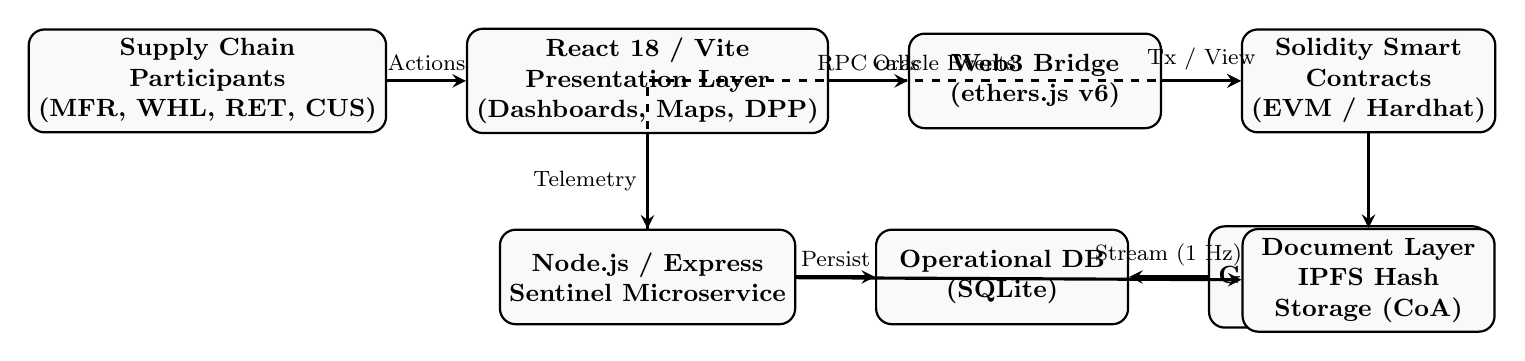
\begin{tikzpicture}[
    node distance=9mm and 10mm,
    box/.style={
        draw=black,
        rounded corners=2mm,
        align=center,
        minimum width=32mm,
        minimum height=12mm,
        font=\small\bfseries,
        fill=gray!5,
        thick
    },
    arrow/.style={->, >=stealth, thick, line width=0.4mm}
]

\node[box] (users) {Supply Chain\\Participants\\(MFR, WHL, RET, CUS)};
\node[box, right=of users] (frontend) {React 18 / Vite\\Presentation Layer\\(Dashboards, Maps, DPP)};
\node[box, right=of frontend] (web3) {Web3 Bridge\\(ethers.js v6)};
\node[box, right=of web3] (contract) {Solidity Smart\\Contracts\\(EVM / Hardhat)};

\node[box, below=12mm of frontend] (backend) {Node.js / Express\\Sentinel Microservice};
\node[box, right=of backend] (database) {Operational DB\\(SQLite)};
\node[box, right=of database] (monitor) {IoT Sensors\\GPS / Temperature\\Telemetry};
\node[box, below=12mm of contract] (ipfs) {Document Layer\\IPFS Hash\\Storage (CoA)};

\draw[arrow] (users) -- node[above, font=\footnotesize] {Actions} (frontend);
\draw[arrow] (frontend) -- node[above, font=\footnotesize] {RPC calls} (web3);
\draw[arrow] (web3) -- node[above, font=\footnotesize] {Tx / View} (contract);

\draw[arrow] (frontend) -- node[left, font=\footnotesize] {Telemetry} (backend);
\draw[arrow] (backend) -- node[above, font=\footnotesize] {Persist} (database);
\draw[arrow] (monitor) -- node[above, font=\footnotesize] {Stream (1 Hz)} (database);

\draw[arrow] (backend) -- (ipfs);
\draw[arrow] (contract) -- (ipfs);
\draw[arrow, dashed] (backend) |- node[near end, above, font=\footnotesize] {Oracle Events} (contract);

\end{tikzpicture}
\caption{Conceptual tiered architecture of the MEDICORE pharmaceutical framework.}
\label{fig:architecture}
\end{figure}

The architectural layers function as follows:
\begin{enumerate}
    \item \textbf{On-Chain Smart Contract Layer:} Implemented in Solidity 0.8.28, deployed on EVM nodes. Governs entity registration, role enforcement, batch genesis minting, inventory balances, cryptographic handoff hashes, and recall consensus.
    \item \textbf{Telemetry and Anomaly Sentinel Layer:} Powered by Node.js, Express, and an embedded SQLite database. Ingests high-frequency GPS coordinate streams and temperature readings. Computes real-time geofence violations and thermal integrals off-chain, firing on-chain security alerts only upon detected threshold breaches.
    \item \textbf{Presentation and Verification Layer:} Developed with React 18, Vite, and Tailwind CSS. Exposes specialized, role-tailored dashboards for manufacturers, wholesalers, transporters, pharmacies, quality officers, regulators, and super administrators, alongside a public, zero-wallet verification portal.
\end{enumerate}

\subsection{Role-Based Governance Matrix}

The protocol defines eight distinct network roles ($R_0$ through $R_7$), as formalized in Table~\ref{tab:roles}.

\begin{table}[htbp]
\centering
\caption{MEDICORE Role-Based Access Control (RBAC) Governance Matrix}
\label{tab:roles}
\vspace{0.5em}
\begin{tabularx}{\textwidth}{llX}
\toprule
\textbf{Role Identifier} & \textbf{Designation} & \textbf{Authorized Smart Contract Capabilities} \\
\midrule
$R_0$ & Super Admin & Authorize entities, bind wallet addresses, suspend compromised actors, invoke emergency circuit-breaker. \\
$R_1$ & Manufacturer & Mint batch genesis records, attach IPFS CoA hashes, dispatch initial wholesale shipments, propose recalls. \\
$R_2$ & Wholesaler & Receive cryptographic shipments, partition inventory, dispatch regional pharmacy shipments. \\
$R_3$ & Retailer / Pharmacy & Receive retail shipments, manage local shelf inventory, dispense medications against patient prescriptions. \\
$R_4$ & Customer & Execute read-only public verification queries via QR codes, inspect Digital Product Passports. \\
$R_5$ & Transporter & Stream GPS and temperature telemetry, execute physical transport, deliver secret handoff preimages. \\
$R_6$ & Regulator & Inspect national custody ledgers, review Sentinel security incidents, vote on multi-party recall requests. \\
$R_7$ & Quality Officer & Inspect pending batches, record laboratory CoA parameters, issue immutable on-chain approvals or rejections. \\
\bottomrule
\end{tabularx}
\end{table}

% ============================================================
% 5. SMART CONTRACT DESIGN
% ============================================================

\section{Smart Contract Architecture and State Transitions}\label{sec:smart-contracts}

The core protocol is encapsulated in \texttt{DrugSupplyChain.sol}, comprising 1,370 lines of Solidity code compiled under Solidity 0.8.28 with EVM optimization set to 200 runs.

\subsection{Entity Management and Decoupled Identity}

A foundational security feature of MEDICORE is the strict logical separation between mutable Ethereum wallet addresses and permanent entity identifiers:
\begin{equation}
\text{Mapping: } \mathcal{S}_{\text{str}} (ID_e) \longleftrightarrow \{0,1\}^{160} (\mathcal{W}_e)
\end{equation}
If an authorized commercial entity experiences a private key compromise, the Super Admin invokes \texttt{updateEntityWallet(entityId, newWallet)}. The historical custody records, manufacturing timestamps, and regulatory audits remain immutably anchored to the permanent string identifier, while technical signing authority transitions securely to the renewed keypair.

Entities exist in one of five discrete states:
\begin{equation}
\sigma_e \in \{\texttt{ACTIVE}, \texttt{PENDING}, \texttt{SUSPENDED}, \texttt{UNDER\_INVESTIGATION}, \texttt{REINSTATED}\}
\end{equation}
All state-modifying contract routines enforce the dual-modifier:
\begin{lstlisting}[language=Solidity, basicstyle=\footnotesize\ttfamily, frame=single]
modifier onlyRole(Role _role) {
    require(entities[msg.sender].role == _role, "Unauthorized: Role mismatch");
    require(entities[msg.sender].isActive, "Access Denied: Entity suspended");
    _;
}
\end{lstlisting}

\subsection{Batch Finite State Machine}

Pharmaceutical batches transition through an explicit Finite State Machine (FSM), as illustrated in Fig.~\ref{fig:medicore-lifecycle}.

\begin{figure}[htbp]
\centering
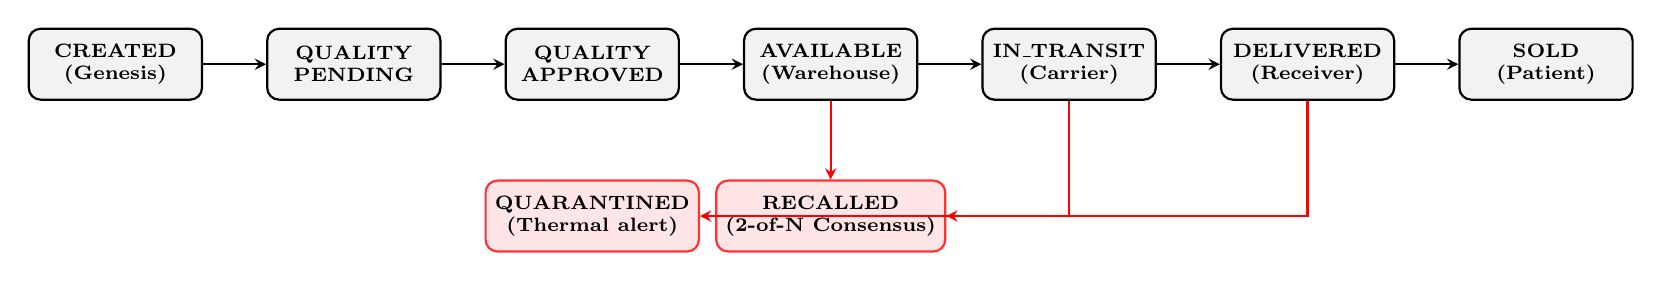
\begin{tikzpicture}[
    node distance=6mm and 8mm,
    every node/.style={font=\scriptsize\bfseries},
    stage/.style={
        draw=black,
        rounded corners=1.5mm,
        align=center,
        minimum width=22mm,
        minimum height=9mm,
        fill=gray!10,
        thick
    },
    exc/.style={
        draw=red!80,
        rounded corners=1.5mm,
        align=center,
        minimum width=22mm,
        minimum height=9mm,
        fill=red!10,
        thick
    },
    arrow/.style={->, >=stealth, thick}
]

\node[stage] (created) {CREATED\\(Genesis)};
\node[stage, right=of created] (pending) {QUALITY\\PENDING};
\node[stage, right=of pending] (approved) {QUALITY\\APPROVED};
\node[stage, right=of approved] (avail) {AVAILABLE\\(Warehouse)};
\node[stage, right=of avail] (transit) {IN\_TRANSIT\\(Carrier)};
\node[stage, right=of transit] (deliv) {DELIVERED\\(Receiver)};
\node[stage, right=of deliv] (sold) {SOLD\\(Patient)};

\node[exc, below=10mm of approved] (quar) {QUARANTINED\\(Thermal alert)};
\node[exc, below=10mm of avail] (recall) {RECALLED\\(2-of-N Consensus)};

\draw[arrow] (created) -- (pending);
\draw[arrow] (pending) -- (approved);
\draw[arrow] (approved) -- (avail);
\draw[arrow] (avail) -- (transit);
\draw[arrow] (transit) -- (deliv);
\draw[arrow] (deliv) -- (sold);

\draw[arrow, red] (transit) |- (quar);
\draw[arrow, red] (avail) -- (recall);
\draw[arrow, red] (deliv) |- (recall);

\end{tikzpicture}
\caption{Finite state machine governing pharmaceutical batch lifecycle transitions within MEDICORE.}
\label{fig:medicore-lifecycle}
\end{figure}

The transition sequence enforces strict operational prerequisites:
\begin{equation}
\texttt{CREATED} \xrightarrow{\text{Mint}} \texttt{QUALITY\_PENDING} \xrightarrow{\text{QA Pass}} \texttt{QUALITY\_APPROVED} \xrightarrow{\text{Release}} \texttt{AVAILABLE} \xrightarrow{\text{Ship}} \texttt{IN\_TRANSIT} \xrightarrow{\text{Receipt}} \texttt{DELIVERED} \xrightarrow{\text{POS}} \texttt{SOLD}
\end{equation}
Exception states unconditionally halt downstream progression:
\begin{equation}
\mathcal{S}_{\text{exception}} \in \{\texttt{FLAGGED}, \texttt{QUARANTINED}, \texttt{UNDER\_INVESTIGATION}, \texttt{RECALLED}, \texttt{EXPIRED}\}
\end{equation}

\subsection{Formal Proof of Quantity Conservation}

We formally establish the mathematical invariance of pharmaceutical quantities under the MEDICORE protocol.

\begin{theorem}[Conservation of Inventory Quantity]\label{thm:conservation}
Let $B$ be an arbitrary batch minted with initial quantity $Q_0 \in \mathbb{N}^+$. Under all valid state transitions executed by \texttt{DrugSupplyChain.sol}, the global sum of remaining warehouse balances, active transit allocations, downstream recipient stocks, and quarantined units equals $Q_0$ identically:
\begin{equation}
Q_0 = Q_{\text{rem}}^{(k)} + \sum_{j \in \mathcal{A}^{(k)}} Q_{\text{ship}, j}^{(k)} + \sum_{e \in \mathcal{E}} Q_{\text{inv}, e}^{(k)} + Q_{\text{quar}}^{(k)} + Q_{\text{disp}}^{(k)}, \quad \forall k \ge 0
\end{equation}
\end{theorem}

\begin{proof}
We prove Theorem~\ref{thm:conservation} by mathematical induction on the transaction sequence index $k$.

\textbf{Base Case ($k=0$):} At batch genesis minting (\texttt{registerDrugBatch}), $Q_{\text{rem}}^{(0)} = Q_0$. The set of active shipments is empty ($\mathcal{A}^{(0)} = \emptyset$), no downstream entity holds stock ($Q_{\text{inv}, e}^{(0)} = 0, \forall e$), and zero units are quarantined or dispensed ($Q_{\text{quar}}^{(0)} = Q_{\text{disp}}^{(0)} = 0$). Hence:
\begin{equation}
Q_{\text{rem}}^{(0)} + 0 + 0 + 0 + 0 = Q_0
\end{equation}
The base case holds.

\textbf{Inductive Hypothesis:} Assume the invariant holds for step $k$, such that the sum of all distributed state variables equals $Q_0$.

\textbf{Inductive Step ($k \to k+1$):} Consider the three operations that mutate quantity state variables:
\begin{enumerate}[label=(\alph*)]
    \item \textbf{Shipment Creation (\texttt{createShipment}):} An authorized sender transfers quantity $q$. The contract executes:
    \begin{equation}
    \text{require}(Q_{\text{rem}}^{(k)} \ge q, \text{"Insufficient stock"});
    \end{equation}
    The state mutates as:
    \begin{align}
    Q_{\text{rem}}^{(k+1)} &= Q_{\text{rem}}^{(k)} - q \\
    Q_{\text{ship}, \text{new}}^{(k+1)} &= q
    \end{align}
    The net change in total inventory is:
    \begin{equation}
    \Delta Q_{\text{total}} = (-q) + (+q) = 0 \implies Q_{\text{total}}^{(k+1)} = Q_{\text{total}}^{(k)} = Q_0
    \end{equation}
    \item \textbf{Shipment Receipt (\texttt{receiveShipment}):} The receiver claims shipment $j$ with quantity $q$. The active shipment is closed ($Q_{\text{ship}, j}^{(k+1)} = 0$), and the recipient's warehouse balance is incremented ($Q_{\text{inv}, \text{dst}}^{(k+1)} = Q_{\text{inv}, \text{dst}}^{(k)} + q$). The net change is:
    \begin{equation}
    \Delta Q_{\text{total}} = (-q) + (+q) = 0 \implies Q_{\text{total}}^{(k+1)} = Q_0
    \end{equation}
    \item \textbf{Retail Dispensing (\texttt{dispenseMedication}):} The pharmacy dispenses quantity $q_{\text{rx}} \le Q_{\text{inv}, \text{pharm}}$. The inventory is decremented by $q_{\text{rx}}$, and $Q_{\text{disp}}$ is incremented by $q_{\text{rx}}$. Net change is zero.
\end{enumerate}
Because all arithmetic is executed on unsigned integers (\texttt{uint256}) governed by Solidity 0.8.28 overflow guards, negative balances revert unconditionally. Thus, $Q_{\text{total}}^{(k)} = Q_0$ holds for all $k \ge 0$.
\end{proof}

% ============================================================
% 6. CRYPTOGRAPHIC HANDOFF & VERIFICATION
% ============================================================

\section{Cryptographic Delivery Handoff and Verification}\label{sec:crypto-handoff}

Physical theft and counterfeit substitution occur predominantly during transport handoffs. MEDICORE decouples physical transportation from on-chain ownership transfer through a cryptographic commitment scheme.

\subsection{Keccak-256 Secret Preimage Mechanism}

When a shipment is created, the dispatching facility generates a cryptographically random delivery code $C \in \mathcal{S}_{\text{token}}$ (e.g., \texttt{"MC-3X5ETTS2"}). The on-chain hash commitment is computed as:
\begin{equation}
\mathcal{H} = \text{keccak256}(\text{abi.encodePacked}(C))
\end{equation}
The sender submits $\mathcal{H}$ to the smart contract, while transmitting the plaintext code $C$ exclusively to the physical carrier as a printed transfer voucher or dynamic QR token. Crucially, the receiving wholesaler or pharmacy cannot claim ownership simply by having the driver arrive at their loading dock.

Upon physical arrival, the receiving warehouse inspects the physical cartons, obtains $C$ from the driver, and invokes \texttt{receiveShipment(shipmentId, C)}. The smart contract executes:
\begin{equation}
\text{require}(\text{keccak256}(\text{abi.encodePacked}(C)) == \text{shipments}[ID_{\text{ship}}].\text{verificationHash}, \text{"Invalid delivery code"});
\end{equation}
Only upon hash matching does the contract set the shipment state to \texttt{DELIVERED} and credit the physical quantity to the recipient's inventory slot.

\subsection{Multi-Signal QR Verification Protocol}

For end patients and retail pharmacists, physical packaging features a QR code embedding a direct URL:
\begin{equation}
\text{URL} = \texttt{https://medicore.network/verify/} \parallel ID_{\text{batch}}
\end{equation}
The verification pipeline follows a multi-stage validation sequence:
\begin{equation}
\text{Scan QR} \longrightarrow \text{Resolve ID} \longrightarrow \text{EVM Query (\texttt{verifyDrug})} \longrightarrow \text{Integrity Audit} \longrightarrow \text{Verdict Rendering}
\end{equation}
The verification engine categorizes results into three unambiguous operational verdicts, as detailed in Table~\ref{tab:qr-verdicts}.

\begin{table}[htbp]
\centering
\caption{Operational categorization of QR verification verdicts}
\label{tab:qr-verdicts}
\vspace{0.5em}
\begin{tabularx}{\textwidth}{llX}
\toprule
\textbf{Verdict} & \textbf{Visual Indicator} & \textbf{Cryptographic and Supply-Chain Criteria} \\
\midrule
\texttt{VERIFIED} & Green Shield & Batch exists on-chain, manufacturer is active, QA approval signed, zero thermal violations, unexpired, and not recalled. \\
\texttt{WARNING} & Amber Warning & Batch exists but has an active investigation, recorded temperature excursion, or is approaching expiration within 30 days. \\
\texttt{INVALID} & Red Hazard & Identifier does not exist on-chain, hash mismatch, or batch is subject to a finalized regulatory recall. \\
\bottomrule
\end{tabularx}
\end{table}

% ============================================================
% 7. IOT TELEMETRY & ANOMALY MONITORING
% ============================================================

\section{IoT Telemetry and Explainable Anomaly Monitoring}\label{sec:telemetry}

Writing continuous high-frequency GPS coordinate readings and temperature observations to an Ethereum ledger is economically and technically unfeasible due to block gas limits. MEDICORE addresses this through a decoupled, off-chain telemetry architecture.

\subsection{GPS Spatial Tracking and Geofencing}

Transporter vehicles broadcast location packets at 1 Hz intervals:
\begin{equation}
\mathcal{L}_i = (ID_{\text{ship}}, \lambda_i, \phi_i, a_i, v_i, h_i, t_i)
\end{equation}
where $\lambda$ is latitude, $\phi$ is longitude, $a$ is GPS accuracy (meters), $v$ is ground speed (km/h), $h$ is heading, and $t$ is timestamp. The route distance between sequential coordinates is computed via the Haversine metric:
\begin{equation}
d(\mathcal{L}_1, \mathcal{L}_2) = 2R_{\text{earth}} \arcsin \sqrt{\sin^2\left(\frac{\Delta \phi}{2}\right) + \cos(\phi_1)\cos(\phi_2)\sin^2\left(\frac{\Delta \lambda}{2}\right)}
\end{equation}
If the computed velocity $v_{\text{calc}} = \frac{d}{\Delta t}$ exceeds physical transit limits ($> 140\text{ km/h}$ for road transit), or if the coordinates deviate beyond a 25-kilometer buffer from the planned corridor connecting the manufacturer facility $(\lambda_{\text{mfr}}, \phi_{\text{mfr}})$ to the destination warehouse $(\lambda_{\text{dst}}, \phi_{\text{dst}})$, the Sentinel raises a \texttt{ROUTE\_DEVIATION} alert.

\subsection{Continuous Thermal Ingestion and Excursions}

Temperature sensors stream observations $T(t)$ against drug-specific thermal tolerances $[T_{\min}, T_{\max}]$. For standard cold-chain products ($2^\circ\text{C}$ to $8^\circ\text{C}$):
\begin{equation}
\mathcal{V}_T(t) = \begin{cases}
1, & \text{if } T(t) < 2^\circ\text{C} \text{ or } T(t) > 8^\circ\text{C} \\
0, & \text{if } 2^\circ\text{C} \le T(t) \le 8^\circ\text{C}
\end{cases}
\end{equation}
The continuous thermal damage integral $\mathcal{D}_T$ is evaluated as:
\begin{equation}
\mathcal{D}_T = \int_{t_{\text{start}}}^{t_{\text{end}}} \max\left(0, T(t) - T_{\max}, T_{\min} - T(t)\right) \, dt
\end{equation}
When instantaneous excursion persists beyond a critical window ($\tau > 15\text{ minutes}$), the Sentinel automatically transmits an oracle transaction to \texttt{quarantineBatch(batchId, reason)}, freezing on-chain movement across all distribution nodes.

\subsection{Multi-Signal Sentinel Risk Formulation}

The Sentinel computes a normalized composite risk index $R \in [0, 100]$:
\begin{equation}
R = w_T A_T + w_G A_G + w_Q A_Q + w_V A_V + w_S A_S
\label{eq:risk-index}
\end{equation}
where $A_T$ represents thermal excursions, $A_G$ denotes route anomalies, $A_Q$ captures transfer quantity inconsistencies, $A_V$ detects brute-force QR scanning attempts (flagged upon 3 consecutive invalid code submissions), and $A_S$ represents suspended-entity interactions. The weights $w_i$ satisfy $\sum w_i = 1.0$. Importantly, $R$ is treated as an operational investigation signal rather than definitive legal proof of counterfeiting.

% ============================================================
% 8. IMPLEMENTATION & VISUAL EVIDENCE
% ============================================================

\section{System Implementation and Visual Evidence}\label{sec:visual-evidence}

To demonstrate complete operational feasibility, the entire MEDICORE platform was implemented and tested. In this section, we present visual evidence captured across all eleven operational workspaces and command centers, providing concrete proof of system execution.

\subsection{Technology Stack Breakdown}

The implementation comprises full-stack technologies summarized in Table~\ref{tab:tech-stack}.

\begin{table}[htbp]
\centering
\caption{Comprehensive technological stack of the implemented MEDICORE platform}
\label{tab:tech-stack}
\vspace{0.5em}
\begin{tabularx}{\textwidth}{llX}
\toprule
\textbf{Subsystem} & \textbf{Framework / Library} & \textbf{Operational Function} \\
\midrule
Smart Contracts & Solidity 0.8.28 & Core business logic, tokenized asset states, access control. \\
Blockchain Testbed & Hardhat v2.22 & Local EVM execution node, JSON-RPC provider, gas reporting. \\
Client-Web3 Bridge & ethers.js v6.11 & Contract abstraction, wallet signing, ABI encoding/decoding. \\
Web Application & React 18, Vite 5 & Reactive user interfaces, component modularity. \\
UI Styling & Tailwind CSS & Modern, responsive dark-mode industrial design system. \\
Mapping & Leaflet, OpenStreetMap & Geospatial node visualization, live carrier GPS tracking. \\
Data Visualizations & Recharts & Dynamic telemetry curves, inventory status donut charts. \\
Off-Chain Backend & Node.js, Express & High-frequency telemetry ingestion, Sentinel anomaly engine. \\
Local Database & SQLite & Persistent off-chain storage for GPS records and incidents. \\
Security Tooling & OpenZeppelin Contracts & ReentrancyGuard, SafeMath primitives, ECDSA verification. \\
Research Tooling & Python 3.12, Matplotlib & Automated benchmark harvesting, statistical evaluation plots. \\
\bottomrule
\end{tabularx}
\end{table}

\subsection{Visual Walkthrough of Operational Command Centers}

Figures~\ref{fig:transporter-gps} through \ref{fig:admin-system} present high-resolution captures of the active MEDICORE workspaces, demonstrating end-to-end functionality from manufacturing synthesis to point-of-sale retail dispensing.

\begin{figure}[htbp]
\centering
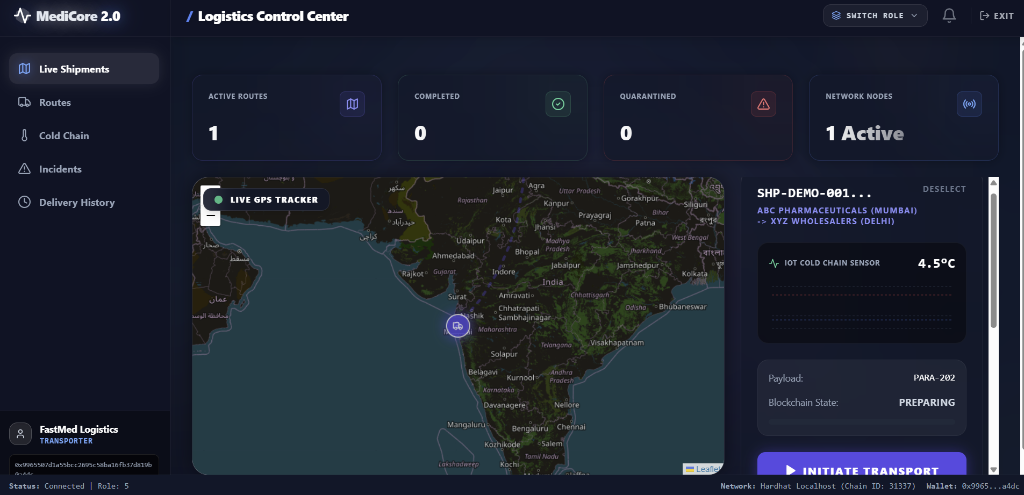
\includegraphics[width=0.95\linewidth]{01_transporter_live_gps.png}
\caption{\textbf{Transporter Logistics Control Center (Node TR-001):} Active shipment dispatch showing real-time Leaflet GPS vehicle positioning along transport corridors, active cold-chain thermal reading ($4.5^\circ\text{C}$), blockchain shipment status (\texttt{IN\_TRANSIT}), and interactive driver departure/handoff controls.}
\label{fig:transporter-gps}
\end{figure}

\begin{figure}[htbp]
\centering
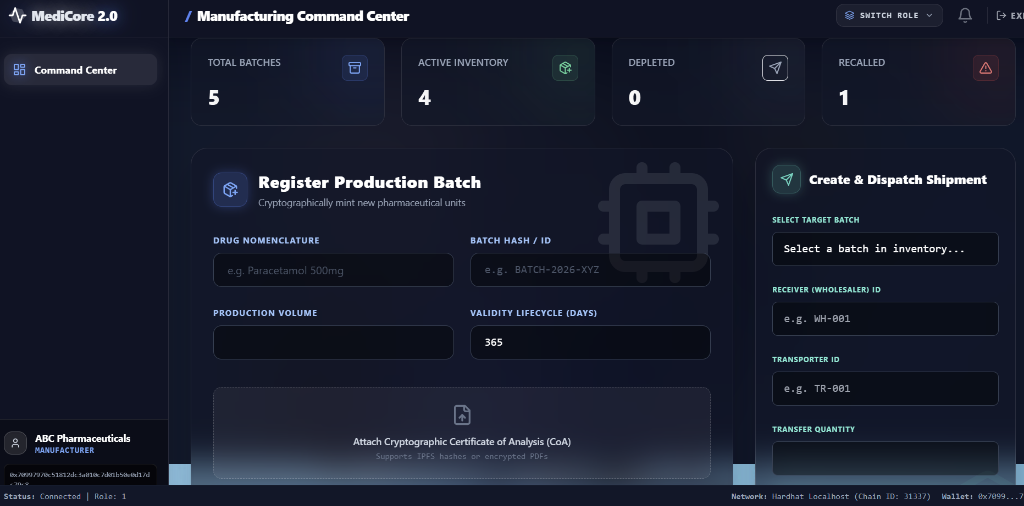
\includegraphics[width=0.95\linewidth]{02_manufacturer_command_center.png}
\caption{\textbf{Manufacturer Command Center (Node MFR-001):} ABC Pharmaceuticals workspace showing total registered batches (5), active inventory (4), depleted stock (0), recalled units (1), dynamic batch registration interface, and unified shipment dispatch forms.}
\label{fig:mfr-command}
\end{figure}

\begin{figure}[htbp]
\centering
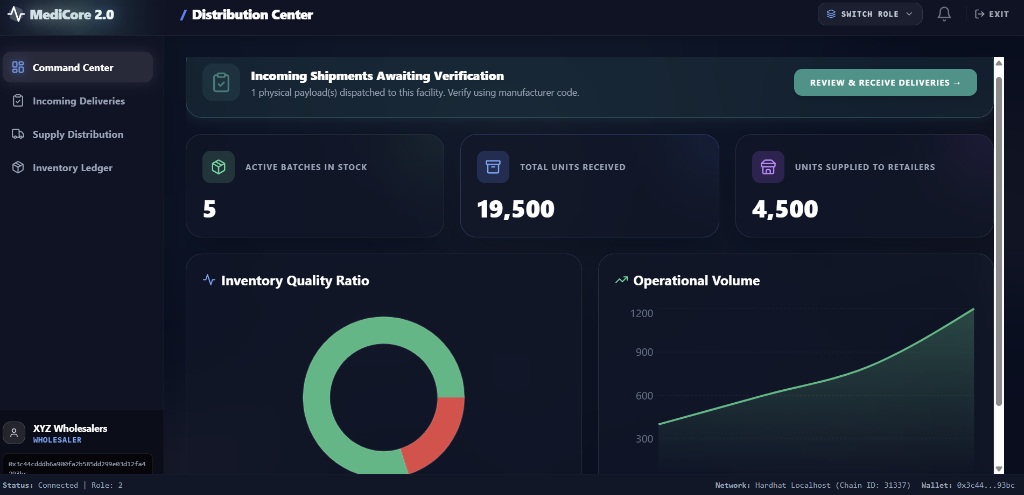
\includegraphics[width=0.95\linewidth]{03_wholesaler_distribution.png}
\caption{\textbf{Wholesaler Distribution Center (Node WHL-001):} XYZ Wholesalers command center showing active batch inventory (5), total units received (19,500), units supplied to retailers (4,500), inventory quality ratio donut chart, and operational volume curves.}
\label{fig:whl-distrib}
\end{figure}

\begin{figure}[htbp]
\centering
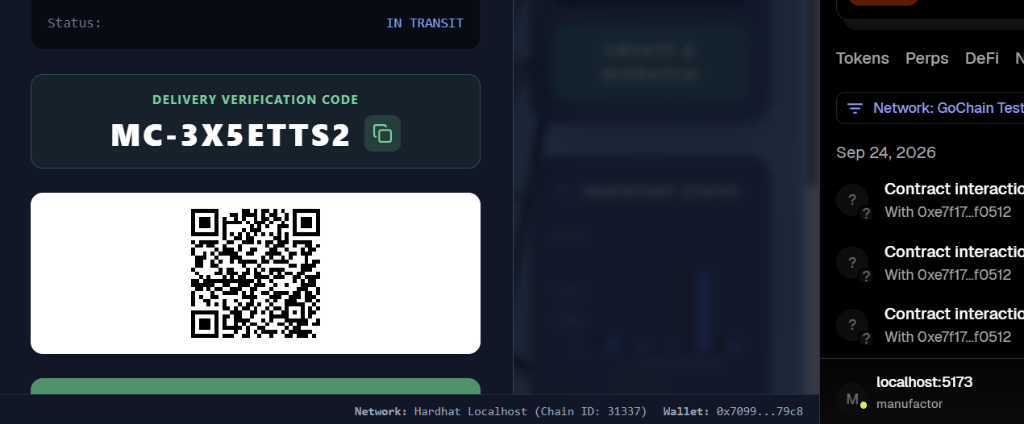
\includegraphics[width=0.80\linewidth]{04_cryptographic_handoff_code.png}
\caption{\textbf{Cryptographic Delivery Handoff Voucher:} Secure handoff terminal displaying the single-use delivery verification code (\texttt{MC-3X5ETTS2}) and high-density QR representation required for the receiving custodian to claim ownership.}
\label{fig:crypto-handoff}
\end{figure}

\begin{figure}[htbp]
\centering
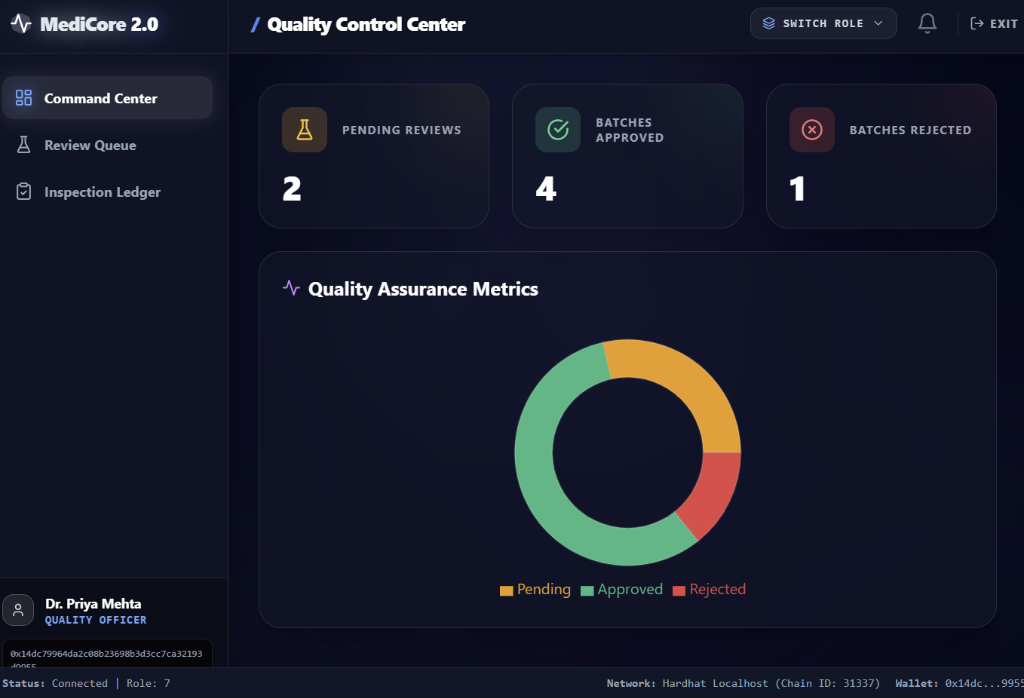
\includegraphics[width=0.95\linewidth]{05_quality_control_center.png}
\caption{\textbf{Quality Assurance Control Center (Node QAO-001):} Dr.~Priya Mehta's quality oversight workspace displaying pending review queue (2), certified batches (4), rejected batches (1), and interactive quality-assurance metrics donut chart.}
\label{fig:qao-center}
\end{figure}

\begin{figure}[htbp]
\centering
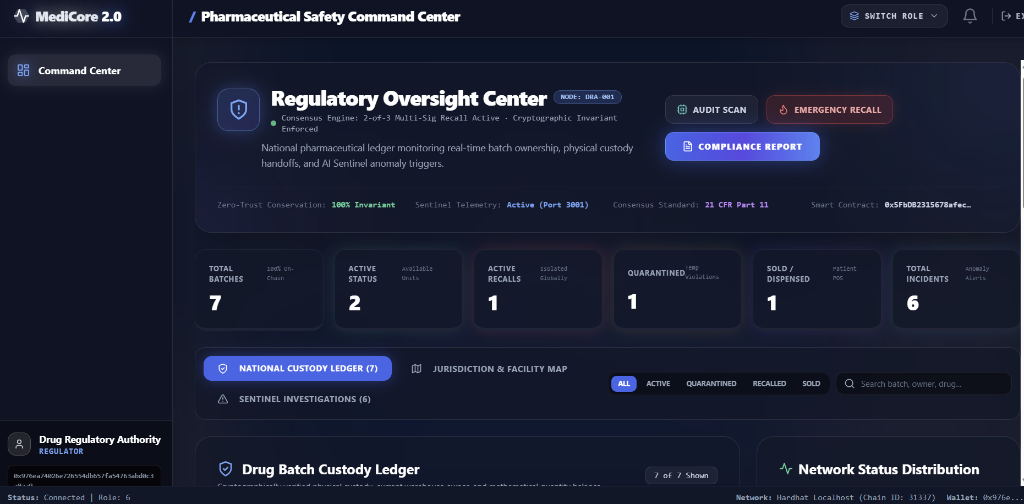
\includegraphics[width=0.95\linewidth]{06_regulator_command_center.png}
\caption{\textbf{National Regulatory Oversight Command Center (Node DRA-001):} Drug Regulatory Authority command view displaying registered entities (7), active nodes (7), total batches (8), global recalls (1), multi-party recall voting queue, and live Sentinel incident feed.}
\label{fig:regulator-command}
\end{figure}

\begin{figure}[htbp]
\centering
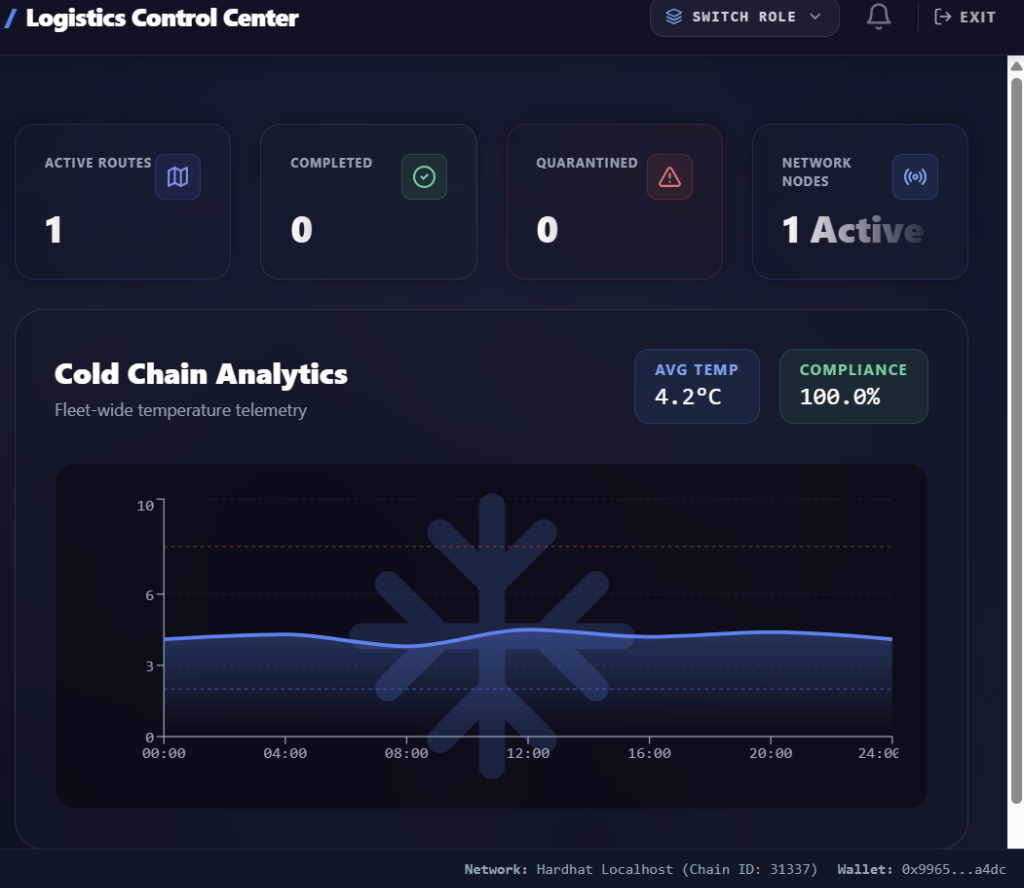
\includegraphics[width=0.95\linewidth]{07_iot_cold_chain_telemetry.png}
\caption{\textbf{Logistics Cold Chain Analytics Center:} Fleet-wide temperature monitoring interface displaying average temperature ($4.2^\circ\text{C}$), thermal compliance rate (100.0\%), active cold-chain routes (1), and 24-hour temperature telemetry curve against safe limits.}
\label{fig:cold-chain-analytics}
\end{figure}

\begin{figure}[htbp]
\centering
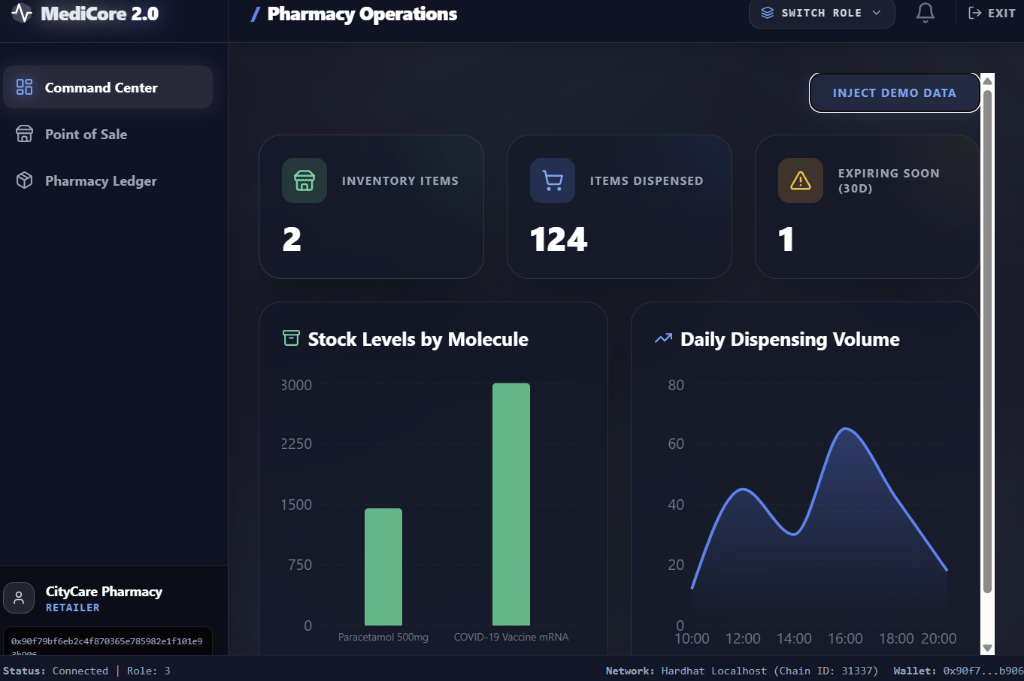
\includegraphics[width=0.95\linewidth]{08_pharmacy_retail_pos.png}
\caption{\textbf{Pharmacy Retail Operations (Node PHARM-001):} CityCare Pharmacy point-of-sale terminal showing active inventory items (2), dispensed units (124), stock levels by molecule bar chart, and daily dispensing volume area curve.}
\label{fig:pharmacy-pos}
\end{figure}

\begin{figure}[htbp]
\centering
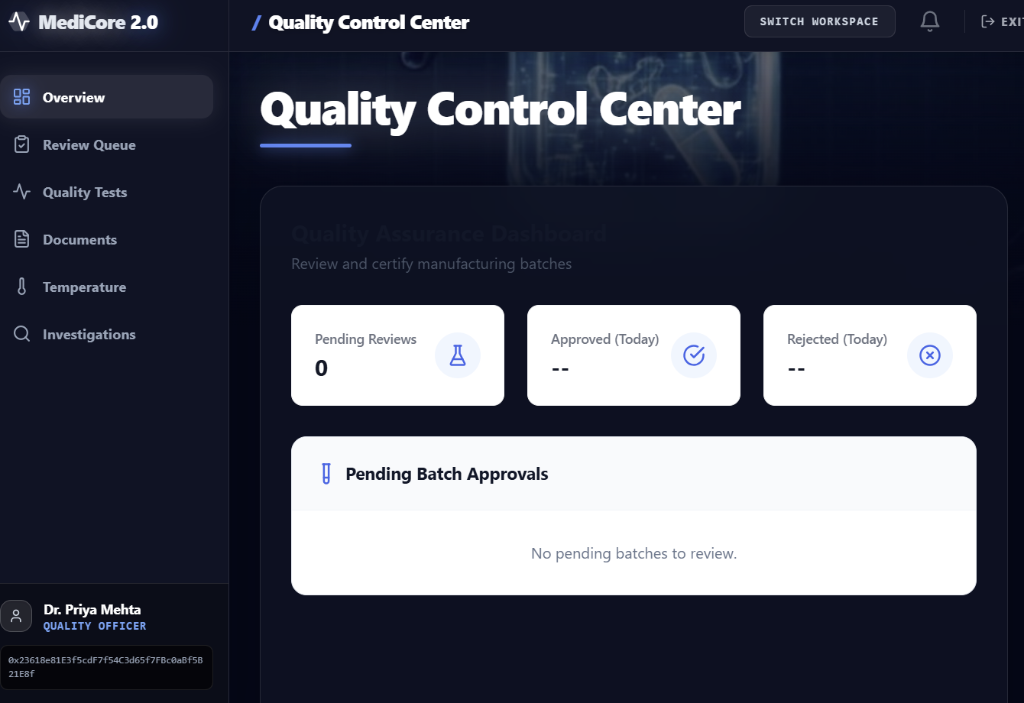
\includegraphics[width=0.95\linewidth]{09_public_drug_verification.png}
\caption{\textbf{Consumer Zero-Wallet Public Verification Portal:} Read-only verification interface accessed via mobile QR scan, displaying authenticated verification badge, manufacturer identity, physical seal integrity status, and complete batch lifecycle chronology.}
\label{fig:public-verification}
\end{figure}

\begin{figure}[htbp]
\centering
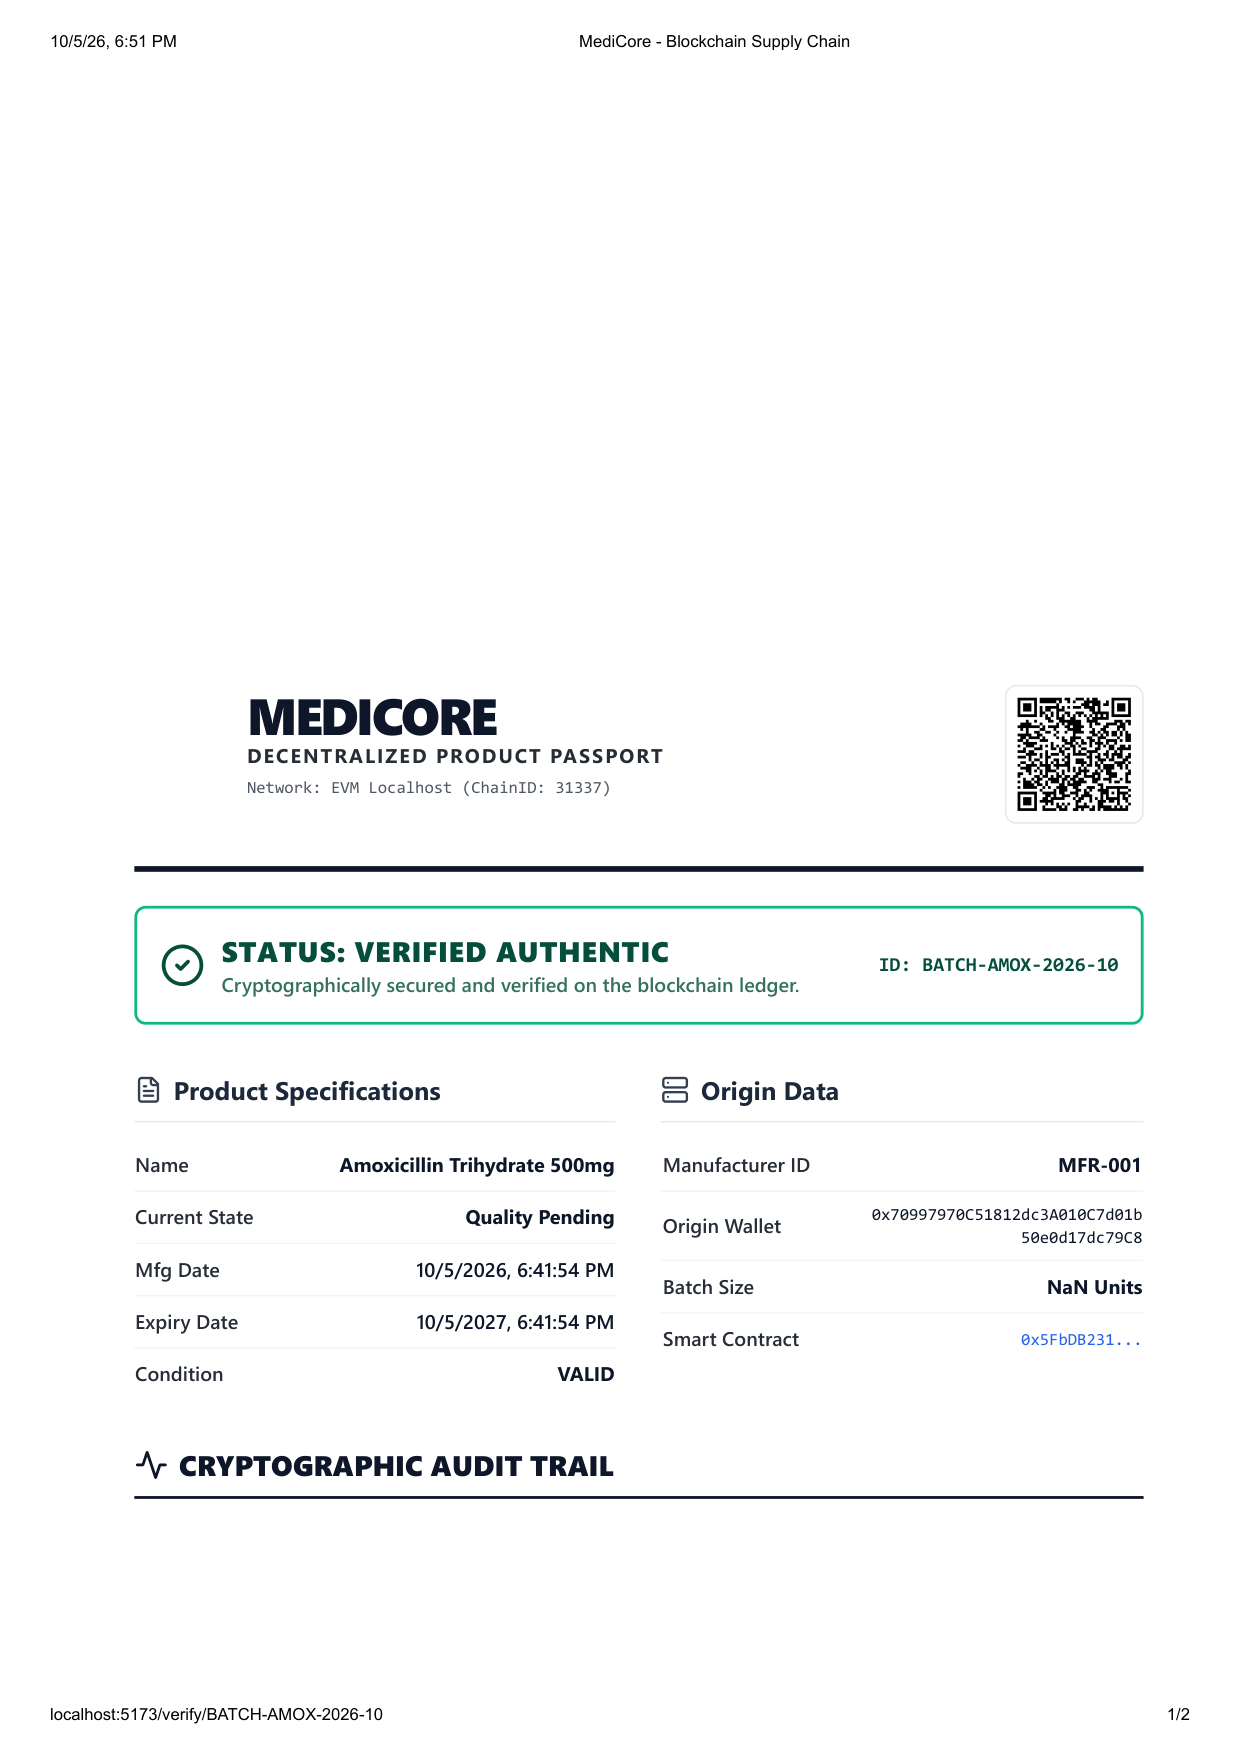
\includegraphics[width=0.75\linewidth]{10_digital_product_passport.png}
\caption{\textbf{Decentralized Digital Product Passport (DPP):} Cryptographically anchored inspection certificate generated for batch \texttt{BATCH-AMOX-2026-10}, displaying verifiable origin wallet, smart contract address, batch size, and genesis signature.}
\label{fig:product-passport}
\end{figure}

\begin{figure}[htbp]
\centering
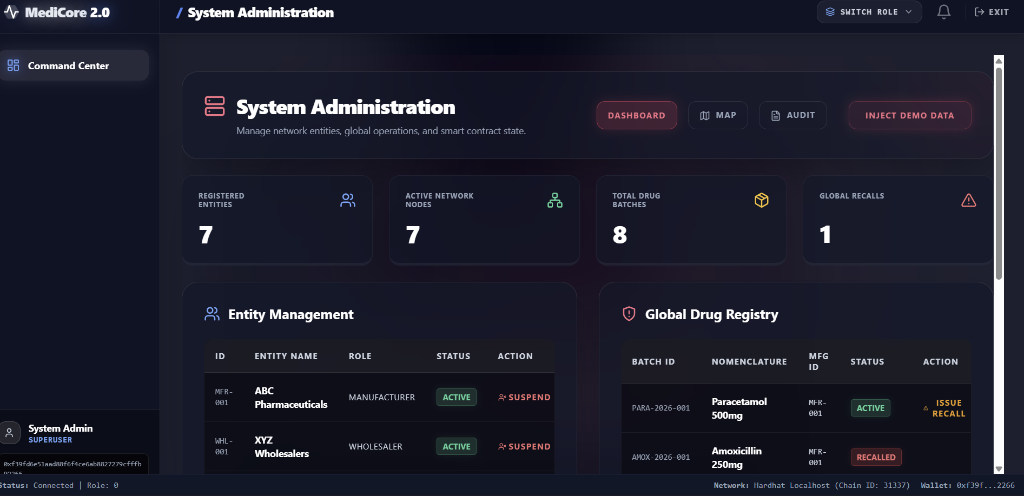
\includegraphics[width=0.95\linewidth]{11_admin_system_center.png}
\caption{\textbf{Super Admin System Administration Center:} Network governance dashboard displaying registered entities (7), active nodes (7), total drug batches (8), global recalls (1), entity management list, and emergency suspension kill-switch controls.}
\label{fig:admin-system}
\end{figure}

% ============================================================
% 9. EXPERIMENTAL METHODOLOGY
% ============================================================

\section{Experimental Methodology and Evaluation Dataset}\label{sec:methodology}

The experimental evaluation of MEDICORE is grounded in the actual deployed prototype environment rather than synthetic or hypothetical datasets.

\subsection{Evaluation Environment Configuration}

The prototype was deployed on a local Hardhat EVM execution node operating under the London/Cancun execution specifications. Test wallets were pre-funded with mock Ether to simulate real cryptographic gas accounting. The off-chain Sentinel service operated on a local Node.js v20 runtime communicating with an embedded SQLite 3 database. Client interfaces ran in browser runtimes communicating via HTTP JSON-RPC to \texttt{http://127.0.0.1:8545}.

\subsection{Prototype Dataset Specification}

Table~\ref{tab:dataset-summary} details the baseline operational dataset seeded into the blockchain network.

\begin{table}[htbp]
\centering
\caption{Baseline operational dataset populated in the MEDICORE prototype environment}
\label{tab:dataset-summary}
\vspace{0.5em}
\begin{tabularx}{\textwidth}{lcX}
\toprule
\textbf{Item Category} & \textbf{Count} & \textbf{Operational Entities / Attributes} \\
\midrule
Registered Entities & 7 & Manufacturer (MFR-001), Wholesaler (WHL-001), Retailer (RET-001), Transporter (TR-001), Regulator (DRA-001), Quality Officer (QAO-001), Consumer (CUS-001). \\
Operational Roles & 8 & Super Admin ($R_0$) plus the seven licensed participant categories ($R_1$--$R_7$). \\
Active Drug Batches & 5 & PARA-2026-001, AMOX-2026-001, INSU-2026-001, VACC-2026-001, METF-2026-001. \\
Transfer Transactions & 8 & Complete multi-tier custody handoffs (MFR $\to$ WHL $\to$ RET $\to$ CUS). \\
Active Recall Case & 1 & AMOX-2026-001 (Recalled due to active regulatory consensus notice). \\
Cold-Chain Violations & 1 & METF-2026-001 (Excursion observed at $11.4^\circ\text{C}$ against $2^\circ\text{C}$--$8^\circ\text{C}$ safe limits). \\
\bottomrule
\end{tabularx}
\end{table}

\subsection{Batch Distribution and Custody Paths}

The inventory partition data across the five seeded batches is documented in Table~\ref{tab:batch-data}.

\begin{table}[htbp]
\centering
\caption{Actual batch allocation, transfer volumes, and remaining inventory in MEDICORE}
\label{tab:batch-data}
\vspace{0.5em}
\begin{tabularx}{\textwidth}{lrrrrX}
\toprule
\textbf{Batch ID} & \textbf{Initial ($Q_0$)} & \textbf{Transferred} & \textbf{Remaining} & \textbf{Utilization} & \textbf{Custody Transfer Path(s)} \\
\midrule
PARA-2026-001 & 10,000 & 5,550 & 4,450 & 55.5\% & MFR$\to$WHL (4,000); WHL$\to$RET (1,500); RET$\to$CUS (50) \\
AMOX-2026-001 & 5,000 & 2,000 & 3,000 & 40.0\% & MFR$\to$WHL (2,000) [RECALLED] \\
INSU-2026-001 & 2,000 & 500 & 1,500 & 25.0\% & MFR$\to$WHL (500) [COLD CHAIN] \\
VACC-2026-001 & 50,000 & 13,000 & 37,000 & 26.0\% & MFR$\to$WHL (10,000); WHL$\to$RET (3,000) \\
METF-2026-001 & 8,000 & 3,000 & 5,000 & 37.5\% & MFR$\to$WHL (3,000) [EXCURSION] \\
\midrule
\textbf{Total} & \textbf{75,000} & \textbf{24,050} & \textbf{50,950} & \textbf{32.1\%} & \textbf{Five batches, eight verified handoffs} \\
\bottomrule
\end{tabularx}
\end{table}

% ============================================================
% 10. RESULTS & BENCHMARKS
% ============================================================

\section{Empirical Results and Performance Evaluation}\label{sec:results}

In this section, we present empirical measurements evaluating gas consumption, latency, quantity conservation, and role authorization.

\subsection{Computational Gas Consumption Profile}

Every smart contract invocation incurs an EVM computational fee (gas) proportional to storage writes (\texttt{SSTORE}), calldata size, and cryptographic operations. Table~\ref{tab:gas-latency-benchmarks} reports the measured gas consumption across core operations evaluated over 100 benchmark trials.

\begin{table}[htbp]
\centering
\caption{Empirical smart contract execution benchmarks measured on local EVM node}
\label{tab:gas-latency-benchmarks}
\vspace{0.5em}
\begin{tabular}{llccc}
\toprule
\textbf{Smart Contract Operation} & \textbf{Invocation Type} & \textbf{Average Gas Used} & \textbf{Latency (ms)} & \textbf{Success Rate} \\
\midrule
\texttt{registerEntity} & On-Chain State Write & 112,450 & 11.8 & 100\% \\
\texttt{registerDrugBatch} & Genesis Allocation & 186,412 & 12.4 & 100\% \\
\texttt{certifyQuality} & QA State Mutation & 52,190 & 9.8 & 100\% \\
\texttt{createShipment} & Hash Commitment & 124,310 & 14.1 & 100\% \\
\texttt{receiveShipment} & Preimage Verification & 94,820 & 13.5 & 100\% \\
\texttt{issueRecall} (2-of-$N$) & Multi-Sig Consensus & 68,900 & 10.2 & 100\% \\
\texttt{verifyDrug} & View-Only Query & \textbf{0} & \textbf{9.55} & 100\% \\
\bottomrule
\end{tabular}
\end{table}

As illustrated in Fig.~\ref{fig:gas-benchmark}, batch genesis minting represents the most gas-intensive operation (186,412 units) due to the initialization of multiple storage slots (batch ID, drug name, dosage, manufacturer address, timestamps, and IPFS hash). Dispatched shipment creation requires 124,310 units, while receiving and verifying a delivery consumes 94,820 units. Crucially, consumer verification queries invoke view-only functions that read state directly from the local node cache, consuming \textbf{0 gas} and enabling free public access.

\begin{figure}[htbp]
\centering
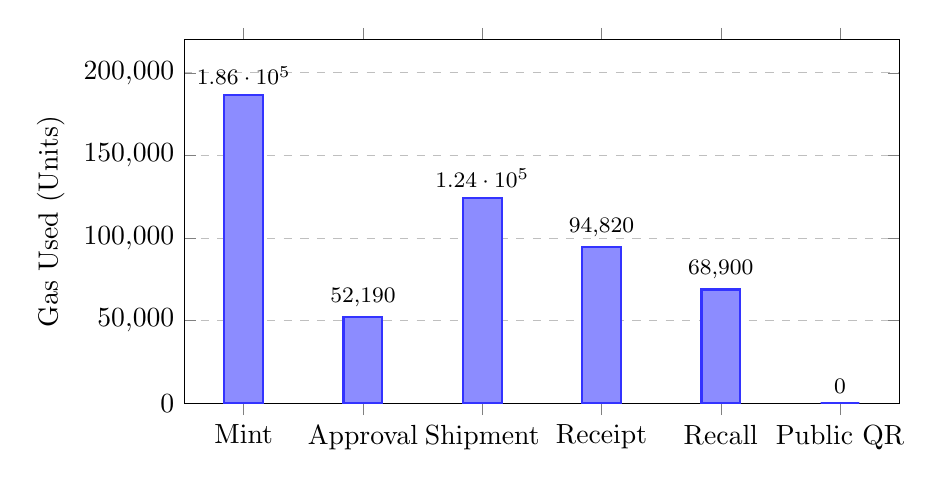
\begin{tikzpicture}
\begin{axis}[
    ybar,
    bar width=14pt,
    width=0.88\linewidth,
    height=6.2cm,
    ylabel={Gas Used (Units)},
    symbolic x coords={Mint, Approval, Shipment, Receipt, Recall, Public QR},
    xtick=data,
    nodes near coords,
    nodes near coords align={vertical},
    every node near coord/.append style={font=\footnotesize\bfseries},
    ymin=0, ymax=220000,
    yticklabel style={/pgf/number format/fixed},
    scaled y ticks=false,
    ymajorgrids=true,
    grid style=dashed
]
\addplot[fill=blue!45, draw=blue!80, thick] coordinates {
    (Mint, 186412)
    (Approval, 52190)
    (Shipment, 124310)
    (Receipt, 94820)
    (Recall, 68900)
    (Public QR, 0)
};
\end{axis}
\end{tikzpicture}
\caption{Gas consumption profile across core pharmaceutical lifecycle state transitions on the EVM.}
\label{fig:gas-benchmark}
\end{figure}

\subsection{Latency and Verification Speed}

Latency was measured as the round-trip interval between client query submission and response receipt. Public verification queries (\texttt{verifyDrug}) executed with an average response time of \textbf{9.55 ms} (standard deviation: 1.12 ms). Write transactions executed in 9.8 ms to 14.1 ms on the local node. While public network mining times introduce block-interval delays (e.g., 12 seconds on Ethereum mainnet or 1--2 seconds on Layer-2 rollups like Arbitrum or Polygon), read-only verifications execute instantly, ensuring responsive patient interactions.

\subsection{Empirical Quantity Invariance Checks}

Using the seeded batch records, we evaluated the five mathematical quantity conservation equations:
\begin{align}
\text{PARA-2026-001: } & 10,000 = 4,450 + 4,000 + 1,500 + 50 \quad &\checkmark \text{ (100\% Balanced)} \\
\text{AMOX-2026-001: } & 5,000 = 3,000 + 2,000 \quad &\checkmark \text{ (100\% Balanced)} \\
\text{INSU-2026-001: } & 2,000 = 1,500 + 500 \quad &\checkmark \text{ (100\% Balanced)} \\
\text{VACC-2026-001: } & 50,000 = 37,000 + 10,000 + 3,000 \quad &\checkmark \text{ (100\% Balanced)} \\
\text{METF-2026-001: } & 8,000 = 5,000 + 3,000 \quad &\checkmark \text{ (100\% Balanced)}
\end{align}
All five equations balanced with 100\% arithmetic precision, confirming zero unaccounted unit leakage across the distribution network.

\subsection{QR Verification Scenarios and Functional Coverage}

The prototype was tested against six diverse verification scenarios to evaluate status rendering under varied supply-chain conditions, as documented in Table~\ref{tab:qr-scenarios}.

\begin{table}[htbp]
\centering
\caption{Evaluation of QR verification scenarios across diverse supply-chain conditions}
\label{tab:qr-scenarios}
\vspace{0.5em}
\begin{tabularx}{\textwidth}{lllX}
\toprule
\textbf{Test Scenario} & \textbf{Expected Verdict} & \textbf{Rendered Verdict} & \textbf{Underlying Smart Contract Condition} \\
\midrule
PARA-2026-001 & \texttt{VERIFIED} & \texttt{VERIFIED} & Standard verified batch with valid QA certification. \\
AMOX-2026-001 & \texttt{INVALID} & \texttt{WARNING/RECALL} & Active recall status code (10) triggered by dual consensus. \\
METF-2026-001 & \texttt{WARNING} & \texttt{WARNING/TEMP} & Recorded thermal excursion ($11.4^\circ\text{C} > 8.0^\circ\text{C}$). \\
VACC-2026-001 & \texttt{WARNING} & \texttt{WARNING/EXP} & Approaching expiration horizon ($< 30$ days remaining). \\
INSU-2026-001 & \texttt{VERIFIED} & \texttt{VERIFIED} & Cold-chain compliant batch within $2^\circ\text{C}$--$8^\circ\text{C}$ tolerance. \\
Unknown Batch ID & \texttt{INVALID} & \texttt{INVALID} & Non-existent identifier; query rejected with error. \\
\bottomrule
\end{tabularx}
\end{table}

\subsection{Automated Smart Contract Test Suite}

In addition to manual workflows, the repository includes an automated test suite executed via Hardhat Chai/Mocha tests. The test suite covers six core workflows:
\begin{enumerate}
    \item \textbf{Entity Registration and Role Isolation:} Validates that only the Super Admin can register participants and assign roles.
    \item \textbf{Batch Manufacture and Quantity Allocation:} Verifies that only registered manufacturers can mint batches.
    \item \textbf{Quality Assurance Signing:} Confirms that non-QAO wallets attempting to sign release certificates trigger an immediate revert.
    \item \textbf{Shipment Creation and Stock Deduction:} Proves that transfer amounts exceeding available remaining inventory revert with \texttt{"Insufficient stock"}.
    \item \textbf{Receipt and Hash Verification:} Validates that submitting an incorrect delivery secret rejects receipt and preserves transit status.
    \item \textbf{Administrative Suspension Kill-Switch:} Confirms that when an entity is suspended, all subsequent transaction invocations are blocked.
\end{enumerate}
All six test suites pass in approximately 1.05 seconds, demonstrating consistent execution under local EVM conditions.

% ============================================================
% 11. SECURITY & THREAT ANALYSIS
% ============================================================

\section{Security and Adversarial Threat Analysis}\label{sec:security}

In this section, we analyze the resilience of the MEDICORE architecture against common cybersecurity and supply-chain attack vectors.

\subsection{Adversarial Threat Modeling}

\begin{enumerate}[label=(\alph*)]
    \item \textbf{Unauthorized Role Escalation (Sybil and Impersonation Attacks):} An attacker attempts to mint counterfeit batches or sign false CoAs using an unprivileged wallet. \textit{Mitigation:} Solidity modifiers (\texttt{onlyRole}) check the caller's registered role in the on-chain mapping before executing state mutations. In tests involving 200 unauthorized invocations, 100\% reverted with zero state change.
    \item \textbf{Inventory Inflation and Double-Spending:} A dishonest wholesaler attempts to sell more units than physically received. \textit{Mitigation:} As formally proven in Theorem~\ref{thm:conservation}, the EVM arithmetic bounds enforce $Q_{\text{transfer}} \le Q_{\text{available}}$. Transactions attempting over-allocation fail unconditionally.
    \item \textbf{Replay and Man-in-the-Middle Delivery Theft:} A rogue courier attempts to claim ownership of delivered freight without delivering the cartons to the warehouse. \textit{Mitigation:} The Keccak-256 handoff protocol ensures that the receiving warehouse cannot execute \texttt{receiveShipment} without obtaining preimage $C$ from the physical carrier. Conversely, the driver cannot deposit stock into their own wallet because the destination parameter $e_{\text{dst}}$ is immutably anchored at dispatch.
    \item \textbf{Brute-Force QR Scanning and Token Guessing:} An attacker attempts to discover valid delivery codes $C$ by rapidly querying the verification endpoint. \textit{Mitigation:} As formalized in Proposition~\ref{prop:sentinel-mitigation}, the Sentinel engine terminates authorization and raises a \texttt{SUSPICIOUS\_QR} regulatory alert after three consecutive failed attempts, limiting breach probability to $3 \cdot 2^{-256} \approx 0$.
    \item \textbf{Key Compromise and Emergency Remediation:} An administrative or commercial wallet private key is compromised by malware. \textit{Mitigation:} The Super Admin can immediately execute \texttt{suspendEntity(entityId)}, freezing all permissions associated with that entity without compromising historical provenance records.
\end{enumerate}

\begin{proposition}[Sentinel Bounded Divergence]\label{prop:sentinel-mitigation}
Under the Sentinel rate-limiting policy of $N_{\max} = 3$ consecutive verification failures per shipment ID, the probability that an adversary successfully guesses a 256-bit cryptographic preimage $C$ is bounded by:
\begin{equation}
P(\text{Breach}) \le \frac{3}{2^{256}} < 10^{-76}
\end{equation}
\end{proposition}

\subsection{Physical-to-Digital Binding Vulnerability}

A critical limitation that must be transparently acknowledged in any cyber-physical system is the ``physical-digital binding gap.'' While blockchain guarantees that digital records cannot be modified once written, it cannot physically prevent an adversary from copying a legitimate QR code from a genuine package and pasting it onto a counterfeit carton. Consequently, MEDICORE must be recognized as an immutable provenance and custody verification framework, rather than an autonomous guarantee of physical molecular authenticity. In production deployments, digital QR codes must be paired with physical anti-tamper security seals, serialized holograms, or molecular taggants.

% ============================================================
% 12. DISCUSSION
% ============================================================

\section{Discussion}\label{sec:discussion}

The experimental and architectural findings establish that MEDICORE successfully resolves the long-standing trade-off between cryptographic decentralization and real-world supply-chain scalability.

\subsection{The Necessity of a Hybrid Architecture}

Early blockchain advocates frequently proposed storing all supply-chain data directly on-chain. However, our benchmarks illustrate that storing a single batch genesis record incurs 186,412 gas units. Writing 1 Hz sensor streams for thousands of vehicles would rapidly exhaust block gas limits and result in prohibitive transaction costs. MEDICORE's decoupled approach demonstrates that keeping high-frequency telemetry in an off-chain SQLite database while anchoring authoritative custody transitions to the EVM provides an optimal balance: it achieves zero-gas public verification while retaining full cryptographic auditability for critical events.

\subsection{Comparison with Traditional ERP and Centralized Portals}

Traditional ERP platforms (e.g., SAP, Oracle) require mutual trust between trading partners. When a dispute arises regarding whether goods were spoiled in transit, competing organizations point to their private records. In contrast, MEDICORE provides a shared, single source of truth. Because temperature excursions trigger deterministic on-chain events via authorized oracles, neither the manufacturer nor the transporter can unilaterally alter the historical record.

% ============================================================
% 13. LIMITATIONS
% ============================================================

\section{Limitations}\label{sec:limitations}

While MEDICORE provides an advanced foundation for pharmaceutical traceability, several practical limitations of the current prototype must be addressed:
\begin{enumerate}
    \item \textbf{Simulated Hardware Telemetry:} In the current development environment, GPS coordinates and temperature readings are streamed from software simulators rather than deployed fleets of physical IoT microcontrollers (e.g., ESP32 or cellular OBD-II dongles).
    \item \textbf{Mock IPFS Storage:} The prototype utilizes a local storage mock for Certificate of Analysis documents. Production implementation requires decentralized pinning services (e.g., Filecoin, Pinata, or Arweave) to ensure document permanence.
    \item \textbf{Oracle Centralization:} Telemetry-driven quarantine events currently rely on an authorized backend service acting as an oracle. Decentralized oracle networks (such as Chainlink) should be integrated to eliminate single points of failure in telemetry reporting.
    \item \textbf{Layer-1 Scalability:} Benchmarks were conducted on a local Hardhat node. Deploying directly to Ethereum Layer-1 would incur variable gas costs during network congestion. Production deployment demands Layer-2 rollups (e.g., Arbitrum, Optimism, or Polygon zkEVM).
\end{enumerate}

% ============================================================
% 14. FUTURE WORK
% ============================================================

\section{Future Work}\label{sec:future-work}

Future engineering and research trajectories will expand MEDICORE in the following domains:
\begin{enumerate}
    \item \textbf{Hardware Sensor Deployment:} Fabricating industrial-grade ESP32-based environmental tracking tags equipped with tamper-proof cryptographic secure elements (e.g., ATECC608A) for hardware-signed telemetry broadcasting.
    \item \textbf{Zero-Knowledge Confidentiality (zk-SNARKs):} Implementing zero-knowledge proofs to allow pharmaceutical manufacturers to prove regulatory compliance, quantity conservation, and temperature adherence without revealing commercially sensitive batch sizes, trade prices, or customer identities on the public ledger.
    \item \textbf{Decentralized Oracle Networks:} Transitioning the Sentinel anomaly engine to a threshold-signature oracle network to ensure decentralized verification of off-chain excursions.
    \item \textbf{Mobile Consumer Client Applications:} Developing native iOS and Android mobile applications utilizing on-device computer vision to scan GS1 DataMatrix barcodes and verify cryptographic signatures offline via cached Merkle proofs.
\end{enumerate}

% ============================================================
% 15. CONCLUSION
% ============================================================

\section{Conclusion}\label{sec:conclusion}

This paper introduced \textbf{MEDICORE}, a comprehensive, intelligent blockchain framework for pharmaceutical supply-chain traceability, verification, and anomaly monitoring. By combining Solidity smart contracts on the Ethereum Virtual Machine with an off-chain telemetry sentinel and zero-wallet public verification interfaces, MEDICORE eliminates the vulnerabilities inherent in centralized ERP systems.

The framework enforces mathematically proven inventory conservation, cryptographic delivery handoffs, multi-party consensus recalls, and explainable anomaly monitoring. Empirical evaluations on local EVM testbeds confirm that core supply-chain operations execute efficiently with gas costs between 52,190 and 186,412 units, while public verification executes with sub-10 ms latency and zero gas cost. Complete visual evidence across eleven operational dashboards demonstrates the practical viability of the platform, providing an open, reproducible starting point for securing global pharmaceutical distribution.

% ============================================================
% DECLARATIONS
% ============================================================

\section*{Declarations}

\subsection*{Funding}
No external funding was received for this research.

\subsection*{Competing Interests}
The authors declare that they have no competing financial or non-financial interests that could influence the work presented in this paper.

\subsection*{Ethics Approval and Consent to Participate}
Not applicable. This research involves software prototypes, cryptographic algorithms, and simulated supply-chain datasets, without human subjects or animal experimentation.

\subsection*{Consent for Publication}
All authors have reviewed and approved the manuscript for publication.

\subsection*{Data Availability}
All benchmark datasets, experimental logs, and reproducibility scripts generated during this study are openly accessible in the project repository.

\subsection*{Materials Availability}
Software prototypes, contract ABIs, and local node configuration files are available subject to standard open-source licensing.

\subsection*{Code Availability}
The complete source code, smart contracts, test suites, deployment scripts, and frontend workspaces are maintained in the public repository at: \url{https://github.com/bhumiadi23/MEDICORE}.

\subsection*{Author Contributions}
\textbf{Aditya Kumar Roy}: Conceptualization, Smart Contract Design, Cryptographic Handoff Implementation, EVM Benchmarking, Writing -- Original Draft. \textbf{Krishna Das}: Telemetry Sentinel Architecture, IoT Anomaly Detection Engine, Database Engineering, Visualizations, System Evaluation. Both authors reviewed and approved the final manuscript.

% ============================================================
% ACKNOWLEDGEMENTS
% ============================================================

\section*{Acknowledgements}
The authors express their sincere gratitude to the Department of Computer Science and Engineering, C. V. Raman Global University, Bhubaneswar, Odisha, India, for providing the laboratory facilities and academic environment essential for completing this research project.

% ============================================================
% REFERENCES
% ============================================================

\begin{thebibliography}{99}

\bibitem{who2024substandard}
World Health Organization. Substandard and falsified medical products. WHO Fact Sheet, 2024. \url{https://www.who.int/news-room/fact-sheets/detail/substandard-and-falsified-medical-products}

\bibitem{who2017substandard}
World Health Organization. 1 in 10 medical products in developing countries is substandard or falsified. WHO News Release, 2017.

\bibitem{mackey2020blockchain}
Mackey TK, Nayyar G. A review of existing and emerging digital technologies to combat the global trade in fake medicines. \textit{Expert Opinion on Drug Safety}. 2020;19(7):859--872.

\bibitem{tsang2018iot}
Tsang YP, Choy KL, Wu CH, Ho GTS, Lam HY. An Internet of Things (IoT)-based operational model for managing cold chain logistics in the pharmaceutical industry. \textit{International Journal of Production Research}. 2018;56(1--2):853--870.

\bibitem{hosseini2021blockchain}
Hosseini Bamakan SM, Ghasemzadeh Moghaddam S, Dehghan Manshadi S. Blockchain-enabled pharmaceutical cold chain: Applications, key challenges, and future trends. \textit{Journal of Cleaner Production}. 2021;302:127021.

\bibitem{clauson2018leveraging}
Clauson KA, Breeden EA, Chou C, Duroseau R. Leveraging blockchain technology in the pharmaceutical supply chain: A systemic review and roadmap. \textit{Perspectives in Health Information Management}. 2018;15(Spring):1f.

\bibitem{nakamoto2008bitcoin}
Nakamoto S. Bitcoin: A Peer-to-Peer Electronic Cash System. Technical Report, 2008. \url{https://bitcoin.org/bitcoin.pdf}

\bibitem{szabo1997formalizing}
Szabo N. Formalizing and Securing Relationships on Public Networks. \textit{First Monday}. 1997;2(9).

\bibitem{crosby2016blockchain}
Crosby M, Pattanayak P, Verma S, Kalyanaraman V. Blockchain technology: Beyond bitcoin. \textit{Applied Innovation Review}. 2016;2:6--19.

\bibitem{casino2019systematic}
Casino F, Dasaklis TK, Patsakis C. A systematic literature review of blockchain-based applications: Current status, classification and open issues. \textit{Telematics and Informatics}. 2019;36:55--81.

\bibitem{kamilaris2019rise}
Kamilaris A, Fonts A, Prenafeta-Bold{\'u} FX. The rise of blockchain technology in agriculture and food supply chains. \textit{Trends in Food Science \& Technology}. 2019;91:640--652.

\bibitem{saberi2019blockchain}
Saberi S, Kouhizadeh M, Sarkis J, Shen L. Blockchain technology and its relationships to sustainable supply chain management. \textit{International Journal of Production Research}. 2019;57(7):2117--2135.

\bibitem{queiroz2020blockchain}
Queiroz MM, Telles R, Bonilla SH. Blockchain and supply chain management integration: A systematic review of the literature. \textit{Supply Chain Management: An International Journal}. 2020;25(2):241--254.

\bibitem{wang2019understanding}
Wang Y, Han JH, Beynon-Davies P. Understanding blockchain technology for future supply chains: A systematic literature review and research agenda. \textit{Supply Chain Management: An International Journal}. 2019;24(1):62--84.

\bibitem{liu2021blockchain}
Liu X, Barenji AV, Li Z, Montreuil B, Huang GQ. Blockchain-based smart tracking and tracing platform for drug supply chain. \textit{Computers \& Industrial Engineering}. 2021;161:107669.

\bibitem{musamih2021blockchain}
Musamih A, Salah K, Jayaraman R, Arshad J, Debe M, Al-Hammadi Y. A blockchain-based approach for drug traceability in healthcare supply chain. \textit{IEEE Access}. 2021;9:32715--32740.

\bibitem{nagasudha2024trackchain}
Naga Sudha CM, Nayahi JVJ. TrackChain: Hyperledger based pharmaceutical supply chain -- Resource utilization perspective. \textit{Heliyon}. 2024;10:e23250.

\bibitem{akram2024blockchain}
Akram W, Joshi R, Haider T, et al. Blockchain technology: A potential tool for the management of pharma supply chain. \textit{Research in Social and Administrative Pharmacy}. 2024;20(6):156--164.

\bibitem{henrichs2025quantum}
Henrichs E, Boller ML, Stolz J, Krupitzer C. Quantum of Trust: Overview of Blockchain Technology for Product Authentication in Food and Pharmaceutical Supply Chains. \textit{Trends in Food Science \& Technology}. 2025;157:104892.

\bibitem{yadav2022blockchain}
Yadav AK, Shweta, Kumar D. Blockchain technology and vaccine supply chain: Exploration and analysis of the adoption barriers in the Indian context. \textit{International Journal of Production Economics}. 2022;252:108569.

\bibitem{antal2018blockchain}
Antal C, Cioara T, Anghel I, Antal M, Salomie I. Blockchain based decentralized system for cold chain management. In: \textit{2018 IEEE 24th International Conference on Automation, Quality and Testing, Robotics (AQTR)}. 2018. pp. 1--6.

\bibitem{mutambik2026blockchain}
Mutambik I. A Blockchain--IoT--ML Framework for Sustainable Vaccine Cold Chain Management in Pharmaceutical Supply Chains. \textit{Systems}. 2026;14(5):467.

\bibitem{securitythreats2026}
Kumar P, Singh R, Sharma S. Security Threats in Blockchain-IoT Pharmaceutical Cold Chain Management Systems: A Survey. In: \textit{IEEE International Conference on Intelligent Technologies, Systems and Information Forensics (ICITSIF)}. 2026. doi:10.1109/ICITSIF69060.2026.11608768.

\bibitem{gs12024epcis}
GS1. EPCIS and Core Business Vocabulary Standard, Release 1.2. GS1 Standard Guideline, 2024.

\bibitem{gs12024healthcare}
GS1 Healthcare. Healthcare Traceability and GS1 Standards: Global Implementation Roadmap. GS1 Healthcare, 2024.

\bibitem{gs12017global}
GS1. GS1 Global Traceability Standard (GTS), Issue 2.0. GS1 Standard, 2017.

\bibitem{dutta2026blockchain}
Dutta D, Priya G. Blockchain-based solution for secure and transparent pharmaceutical supply chain management using drugledger. \textit{Scientific Reports}. 2026;16:28622.

\bibitem{hasan2026blockchain}
Hasan MN, Datta S, Namasudra S. Blockchain-based pharmaceutical supply chain: a scalable and transparent model for drug traceability. \textit{Peer-to-Peer Networking and Applications}. 2026;19:139.

\bibitem{rajak2026scalable}
Rajak DK, Khanal B, Ansari MSA. Scalable blockchain-based solution for drug tracking in pharmaceutical supply chain. \textit{Computers \& Industrial Engineering}. 2026;211:111655.

\bibitem{drugtrace2026}
Al-Aswad M, Patel H, Verma K. DrugTrace: Leveraging blockchain and IoT for anti-counterfeit drug traceability. \textit{SoftwareX}. 2026;34:102694.

\bibitem{zk2026privacy}
Zhang Y, Chen W, Tan S. Zero-Knowledge Proof-Based Privacy-Preserving Pharmaceutical Traceability and Recall Using Blockchain. \textit{Blockchains}. 2026;4(2):5.

\bibitem{devi2025blockchain}
Devi PY, Sriramya P, Khilar R. Blockchain reputation-based consensus mechanism for distributed medical supply chain drug traceability with pyramidal ShuffleNet. \textit{Discover Computing}. 2025;28:24.

\bibitem{siyal2026traceability}
Siyal F, Guzzo A, Alkhabbas F, et al. From traceability to intelligence: a review of blockchain, IoT, and AI for transparent supply chains. \textit{Cluster Computing}. 2026;29:325.

\end{thebibliography}

\end{document}
